\documentclass[10pt,a4paper]{article}
\usepackage[utf8]{inputenc}

\usepackage{amsmath}
\usepackage{amsfonts}
\usepackage{amssymb}
\usepackage{graphicx}
\usepackage{listings}
\usepackage[margin=1.0in]{geometry}
\usepackage{caption}
\usepackage{subcaption}
\usepackage{float}
\usepackage[utf8]{inputenc}
\usepackage{refstyle}


\lstset{numbers=left,
	title=\lstname,
	numberstyle=\tiny, 
	breaklines=true,
	tabsize=4,
	language=Python,
	morekeywords={with,super,as},,
	frame=single,
	basicstyle=\footnotesize\tt,
	commentstyle=\color{comment},
	keywordstyle=\color{keyword},
	stringstyle=\color{string},
	backgroundcolor=\color{background},
	showstringspaces=false,
	numbers=left,
	numbersep=5pt,
	literate=
		{æ}{{\ae}}1
		{å}{{\aa}}1
		{ø}{{\o}}1
		{Æ}{{\AE}}1
		{Å}{{\AA}}1
		{Ø}{{\O}}1
	}
\usepackage{setspace}
\doublespacing
\usepackage{bm}
\usepackage{hyperref}

\begin{document}

\begin{center}
{\LARGE\bf
FYS4150\\
Project 4, deadline November 15.
}
 
\includegraphics[scale=0.075]{uio.png}\\
Author: Robin D. Kifle,
University of Oslo, Autumn 2017

\vspace{3cm}
{\LARGE\bf
Abstract
}
\end{center}
We have made a c++ program to calculate some thermodynamic variables for a square lattice using the Ising model. The variables have been used for plots and further calculations in MATLAB. The outputs have shown to be sensitive to temperature, while the initial configuration of the lattice does not matter much. The energy, magnetization, specific heat and susceptibility stays close to the same for each spin for increasing lattice sizes. The critical temperature, showing a phase shift, is found at the same temperature for our lattice sizes, and is found to be at T=2.3.

\newpage

{\LARGE\bf
Introduction
}\\
In this project we will study phase transitions in magnetic systems. We will use the widely popular square-lattice Ising model in two dimensions, where particles interact with their nearest neighbours to get a magnetic spin of either +1 or -1. This model will be used to find a critical temperature showing a phase shift where the system goes from having magnetic moment to zero magnetic moment We will start off by looking at the simple case of a 2x2 lattice and use this as benchmark calculations for the rest of the project. We will then move on to larger lattices, and eventually compare these results to a more realistic model where the lattice is infinite in size. In this project the emphasis will be on understanding and usage of the Metropolis algorithm, and have a look on its efficiency and precision.
The codes and files used in this project can be found at \url{www.da.com}
\\
\newpage

{\LARGE\bf
Method
}\\
Before starting on the program we need to find analytical expressions for the partition function Z and the corresponding energy values E, the mean magnetization $|M|$, the specific heat $C_v$ and the susceptibility $\chi$ as functions of the temperature T using periodic boundary conditions.\\
The partition function is given by: $$Z = \sum\limits_{i=1}^{M}e^{-\beta E_i}$$
Where M is the total number of configurations,$\beta$ is the inverse temperature given by $\beta = \frac{1}{kT}$ with k as the Boltzmann constant. $E_i$ is the energy for different spin settings given by: $$E=J\sum\limits_{<kl>}^{N}s_ks_l$$ where J is a constant which expresses the strength of the interaction between spins. N is the total number of configurations.
 $<kl>$ expresses that we only look at the nearest neighbours in the lattice. $s_k$ and $s_l$ are the spins of two neighbouring objects. \\
 For now we work with a 2x2 lattice and the Ising model where the spins can only be in two states, giving a total number of $2^4=16$ configurations.

\begin{center}
\begin{table} [H]
\caption{Energy with periodic boundary conditions and magnetization for different spin-configurations} \label{tab:table1}
\centerline{
\begin{tabular}{c|c|c}
Spin configuration & Energy& Magnetization\\
$\uparrow \uparrow$ &-2J&2\\
$\uparrow \downarrow$&2J&0\\
$\downarrow \uparrow$&2J&0\\
$\downarrow \downarrow$&-2J&-2\\
\end{tabular}
}
\end{table}
\end{center}

\noindent From the table above one can observe that the energy is only non-zero on lattices where all objects have the same spin (-8J) and when the diagonals have opposite spin (8J). The magnetization of a 2x2 lattice is only zero when half of the objects have the same spin. We can now calculate the mean energy, the mean absolute magnetization, specific heat and susceptibility with these expressions:\\


Partition function:
$$Z = \sum\limits_{i=1}^{16}e^{-\beta E_i}$$
$$Z = 2e^{8\beta J} + 2e^{-8\beta J}+12$$
$$Z = 4cosh(8\beta J)+12$$

Mean energy:
$$<E> = \frac{1}{Z}\sum\limits_{i=1}^{16}e^{-\beta E_i}E_i$$
$$\sum\limits_{i=1}^{16}e^{-\beta E_i}E_i = -16J(e^{8\beta J}-e^{-8\beta J})=-32Jsinh(8\beta J)$$
$$<E>=-\frac{8J}{cosh(8\beta J)+3}sinh(8\beta J)$$

Mean absolute magnetization:

$$<|M|>=\frac{1}{Z}\sum\limits_{i=1}^{16}e^{-\beta E_i}|M_i|$$
$$\sum\limits_{i=1}^{16}e^{-\beta E_i}|M_i|=8e^{8\beta J}+16$$
$$<|M|>=\frac{2e^{8\beta J}+4}{cosh(8\beta J)+3}$$

Specific heat:
$$C_v = \frac{\beta}{T}(<E^2>-<E>^2)$$
$$<E>^2=\frac{64J^2}{(cosh(8\beta J)+3)^2}sinh^2(8\beta J)$$
\begin{center}
$<E^2>=\frac{1}{Z}\sum\limits_{i=1}^{16}e^{-\beta E_i}E_i^2$ = $\frac{64J^2}{cosh(8\beta J)+3}cosh(8\beta J)$\\
$\rightarrow$
$C_v = \frac{64\beta J^2}{T(cosh(8\beta J)+3)^2}(3cosh(8\beta J)+1)$
\end{center}

Susceptibility:
$$\chi=\beta(<|M|^2>-<|M|>^2)$$
\begin{center}
$<|M|^2>=\frac{1}{Z}\sum\limits_{i=1}^{16}e^{-\beta E_i}M_i^2$ = $\frac{8e^{8\beta J}+8}{cosh(8x)+3}$\\
$\rightarrow$
$\chi = \beta(\frac{8e^{8\beta J}+8}{cosh(8\beta J)+3}-\frac{(2e^{8\beta J}+4)^2}{(cosh(8\beta J)+3)^2})$\\
\end{center}
\noindent Notice that the terms in $C_v$ and $\chi$, $<E^2>-<E>^2$ and $<|M|^2>-<|M|>^2$, respectively, are the variance of the energy and variance of the magnetization.\\
\\
As mentioned, we will use the Metropolis algorithm. This algorithm can be described in ten steps:\begin{enumerate}
\item Establish an initial matrix with size $L \times L$ and compute the energy.
\item Position yourself at a random point in the lattice and flip one spin.
\item Compute the energy for this new state.
\item Compute $\vartriangle E$ 
\item If the energy is lowered, accept the new configuration and jump to step 9
\item If the energy is increased, compare $w=e^{-\beta \vartriangle E}$ with a random number.
\item If the random number is bigger than $w$, reject the new configuration and jump back to step 2.
\item If the random number is smaller or equal to $w$, accept the new configuration. 
\item Update expectation values
\item Repeat $L \times L$ times to let every lattice point get a chance to get picked.
\end{enumerate}
\hfill{Hjorth-Jensen., 2015}\\

\noindent From our simulations for a LxL lattice with L=20, L=40, L=60, L=80, L=100, we can find analytical values for the critical temperature $T_c(L)$ at the maximum values for the plots. We can then use these values to find a value for the critical temperature in the thermodynamic limit L$\rightarrow \infty$ using the expression: $$T_c(L)-T_c(L=\infty)=aL^{-1/\nu}$$
Where $a$ is a constant and we use $\nu=1$. We set $L^{-1}=X$ and solve the equation $T_c(L)=aX+T_c(L=\infty)$ using Matlabs' least squares solver.\\



\newpage
{\LARGE\bf
Results
}\\
\begin{center}
\begin{table} [H]
\caption{Analytical and numerical solutions for a random initial matrix} \label{tab:table2}
\centerline{
\begin{tabular}{c|c|c|c}
& Analytical& Numerical& MC cycles\\
$<E>$&-7.983928&-7.98472& 10.000\\
$<|M|>$&3.994643&3.99494& 10.000\\
$C_v$&0.128329&0.122007& 100.000\\
$\chi$&0.016043&0.015054& 100.000\\
\end{tabular}
}
\end{table}
\end{center}
Starting with a 2x2 matrix with a random configuration,
after only 10.000 Monte Carlo cycles the numerical solutions for the mean energy and the mean magnetization are close to the values found analytical. They are only off by a value of $10^{-3}$. To get the same magnitude of agreement for the specific heat and susceptibility, 100.000 Monte Carlo cycles was needed. For fewer than 10.000 Monte Carlo cycles the values are irregular.


\begin{figure}[H]
\centerline{
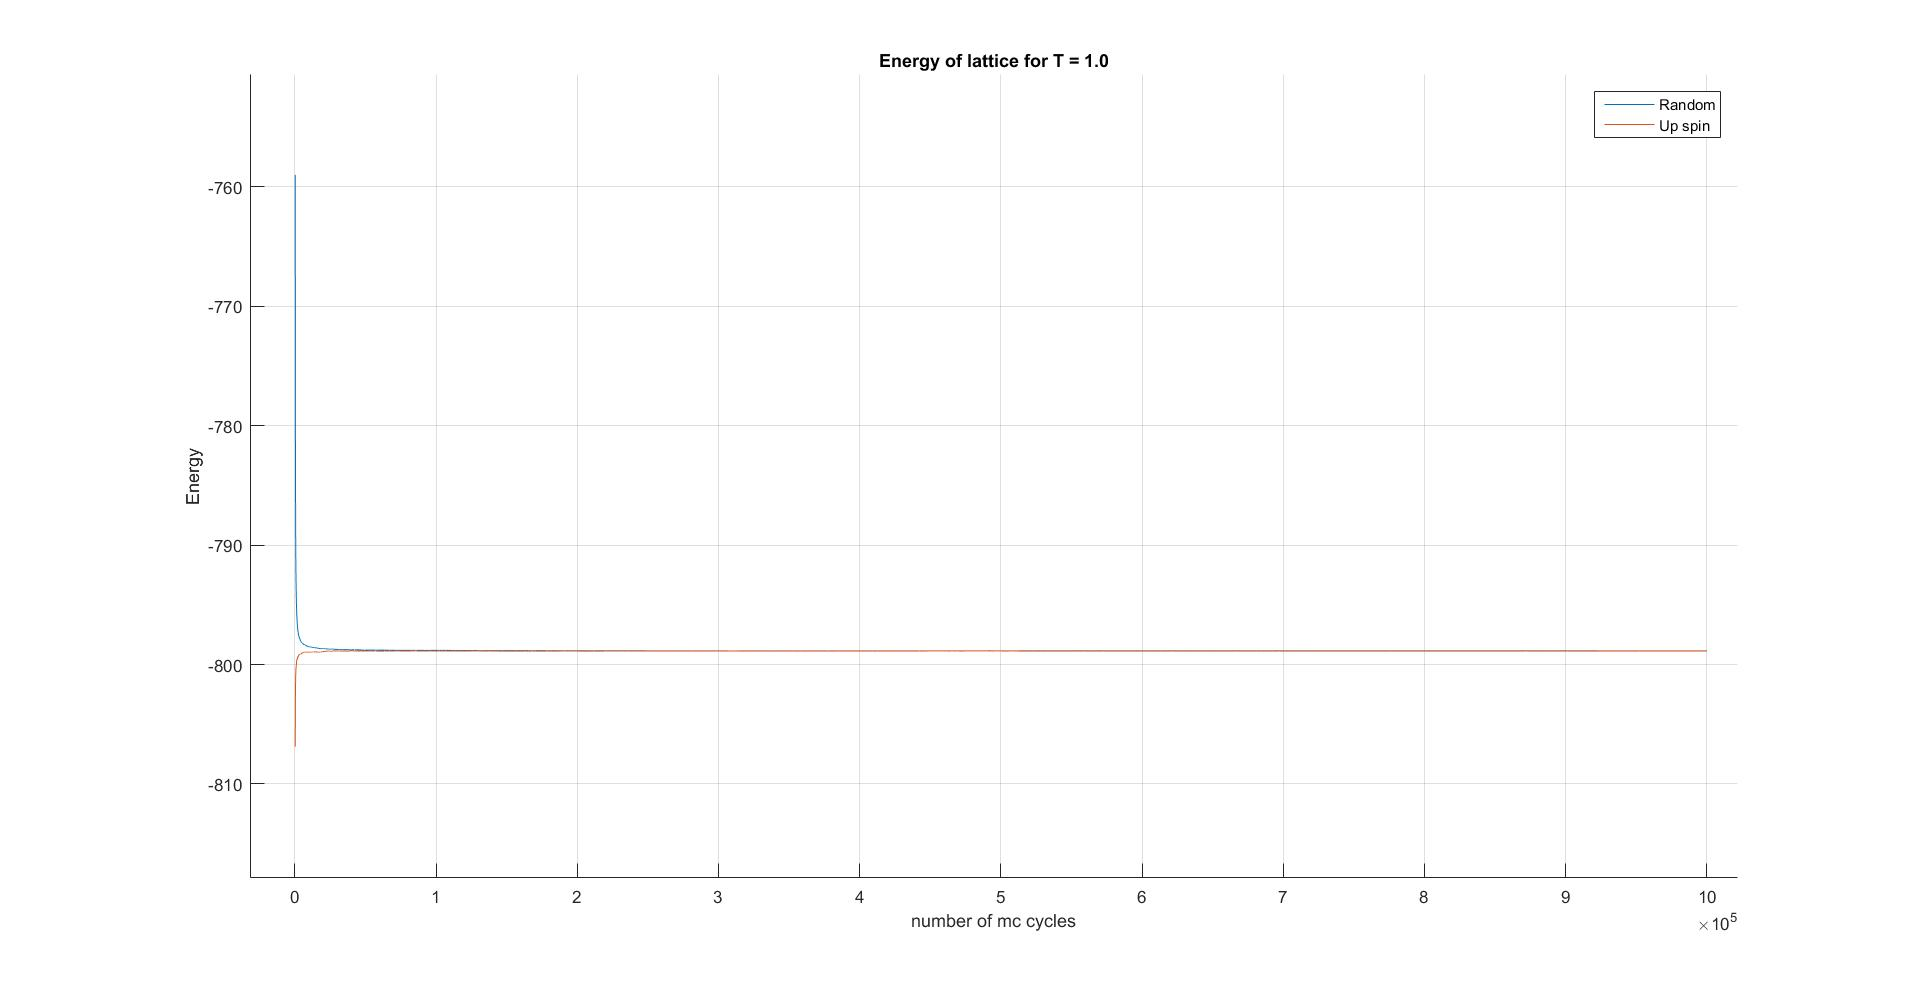
\includegraphics[scale=0.15]{energy1T}
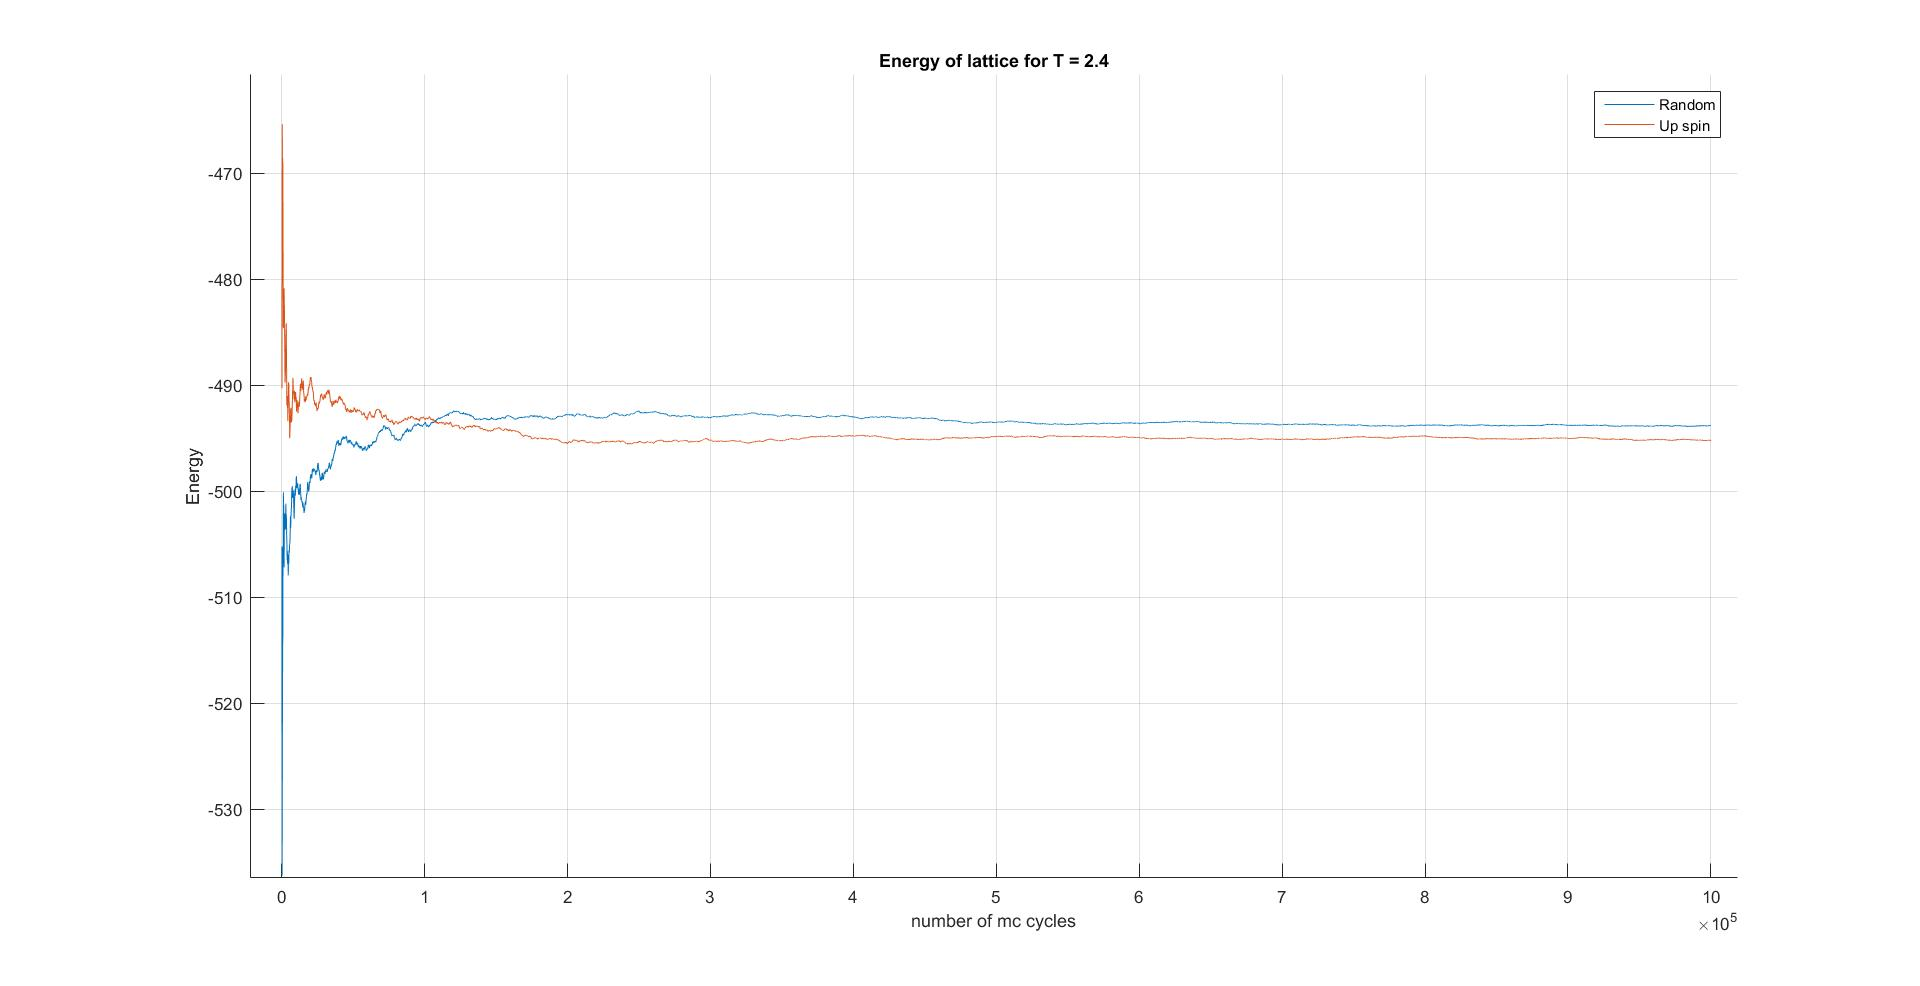
\includegraphics[scale=0.15]{energy24T}
}
\caption{Energy vs. Monte Carlo cycles for random- and up-spin oriented matrix with T=1.0 and T=2.4, respectively}
\label{fig:energy}
\end{figure}
\noindent From figure \ref{fig:energy} and we notice that after some amount of Monte Carlo cycles the random- and up-spin initial matrices converges to the same energy equilibriums. For T=1 the equilibrium is reached after about $2*10^4$ Monte Carlo cycles with a value of -800, or -2 per spin. The up-spin initial matrix reaches equilibrium more promptly than the random initial matrix as it starts from the steady state. For T=2.4 the energy oscillates more, and the equilibrium is reached after about $10^5$ cycles with a value of -495, or  -1.2375 per spin. This oscillation is expected as there is more energy in the system. At T=2.4 the up-spin initial matrix does not start from a steady state and needs more cycles before reaching the equilibrium compared to the system with T=1.

\begin{figure}[H]
\centerline{
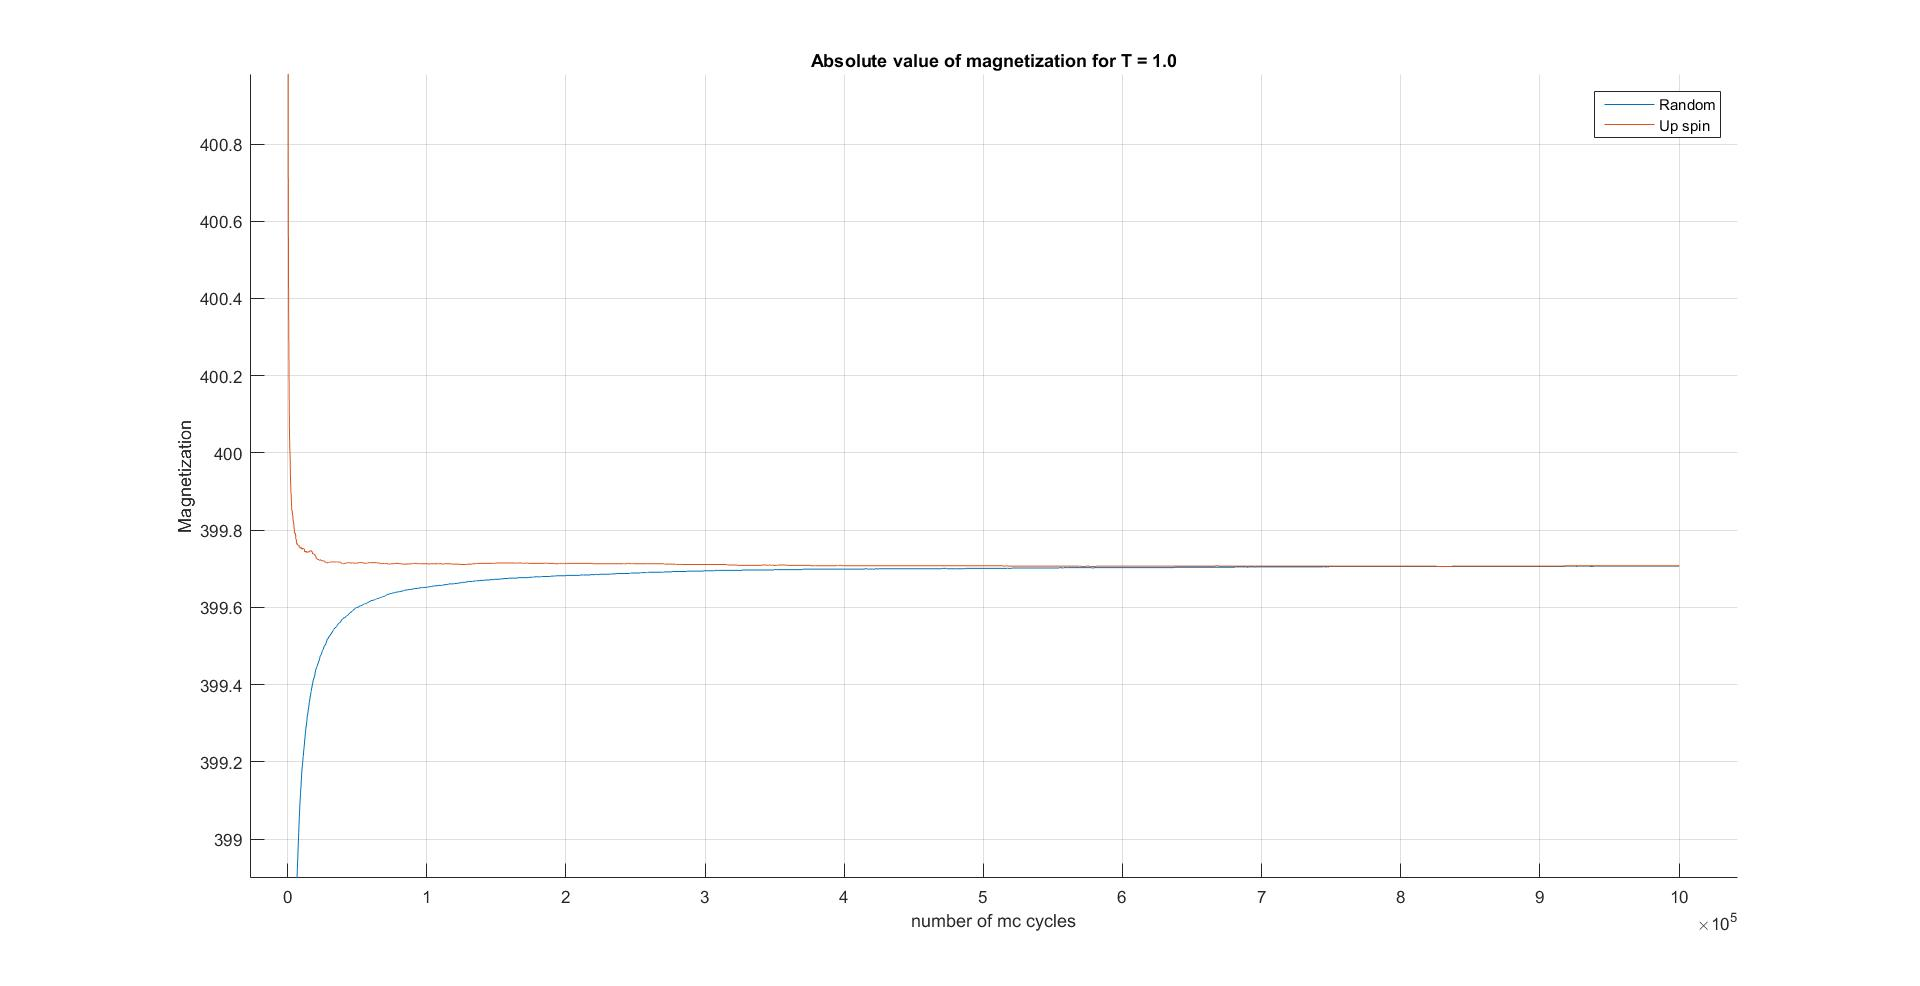
\includegraphics[scale=0.15]{absmag1T}
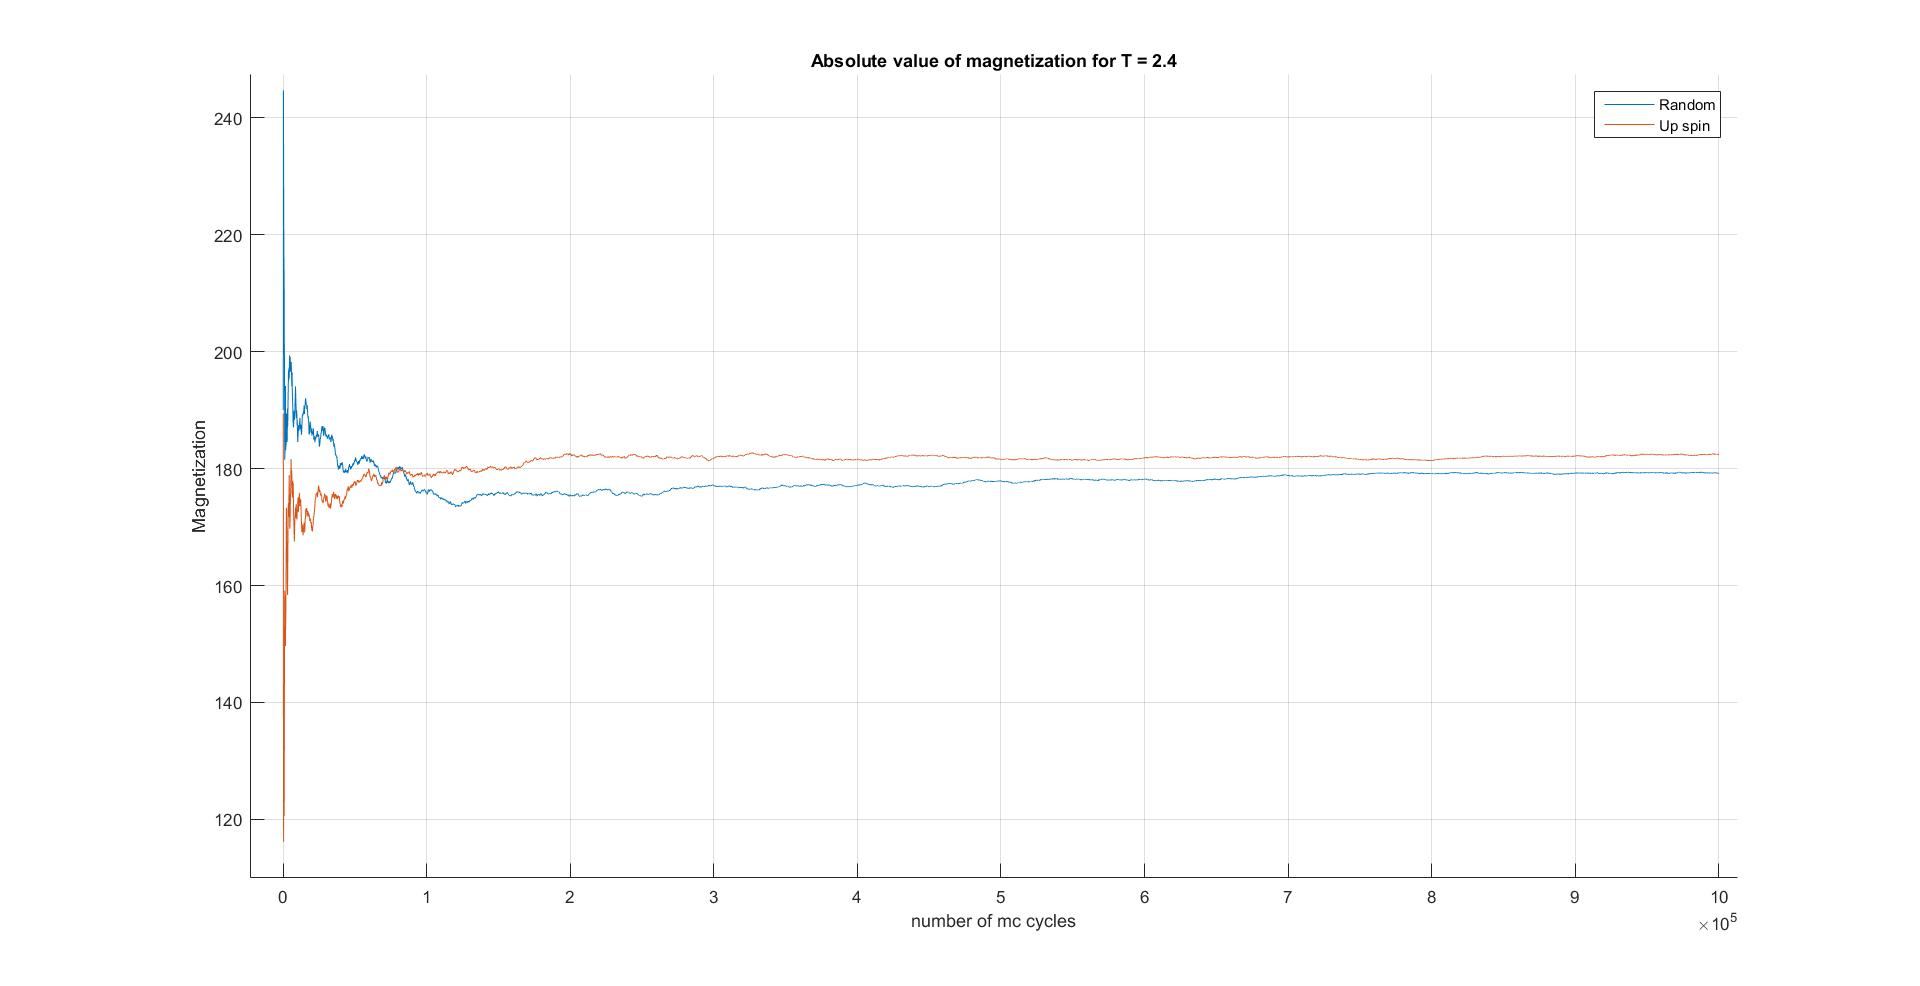
\includegraphics[scale=0.15]{absmag24T}
}
\caption{Absolute magnetization vs. Monte Carlo cycles for random- and up-spin oriented matrix with T=1.0 and T=2.4, respectively}
\label{fig:absmagn}
\end{figure}

\begin{figure}[H]
\centerline{
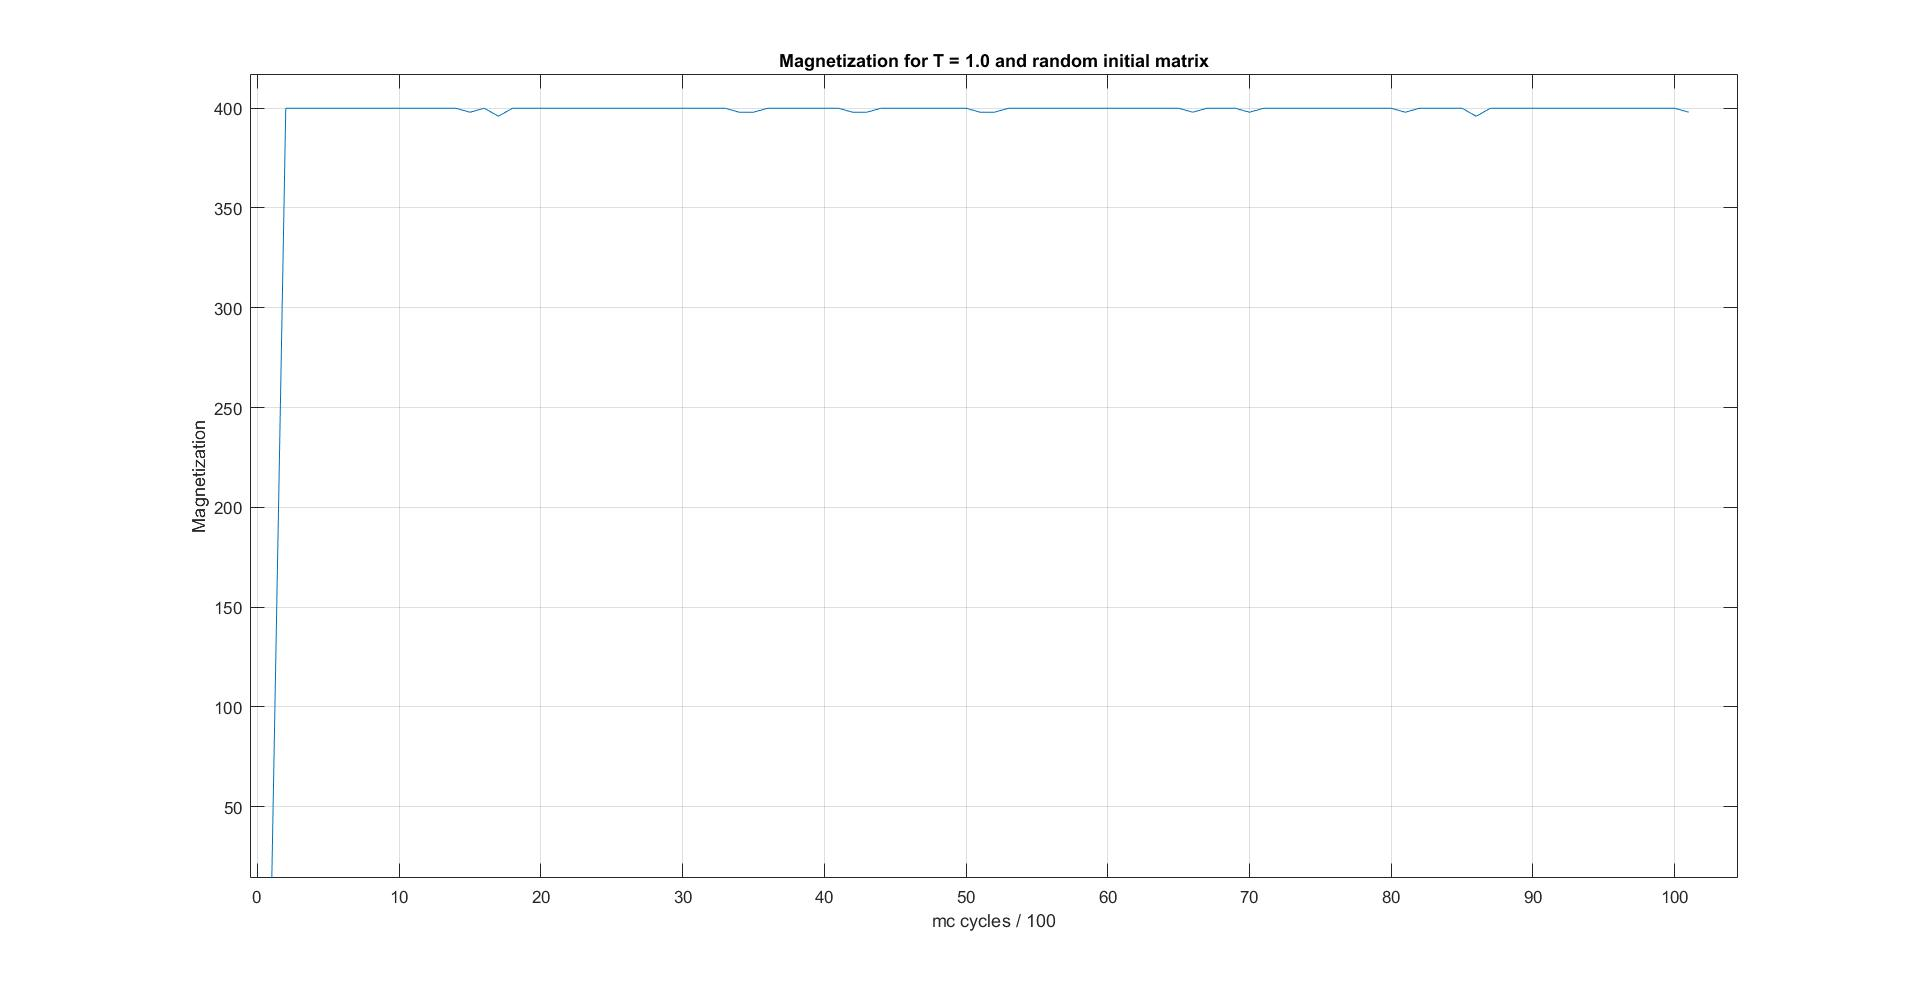
\includegraphics[scale=0.15]{magnetizationT1random}
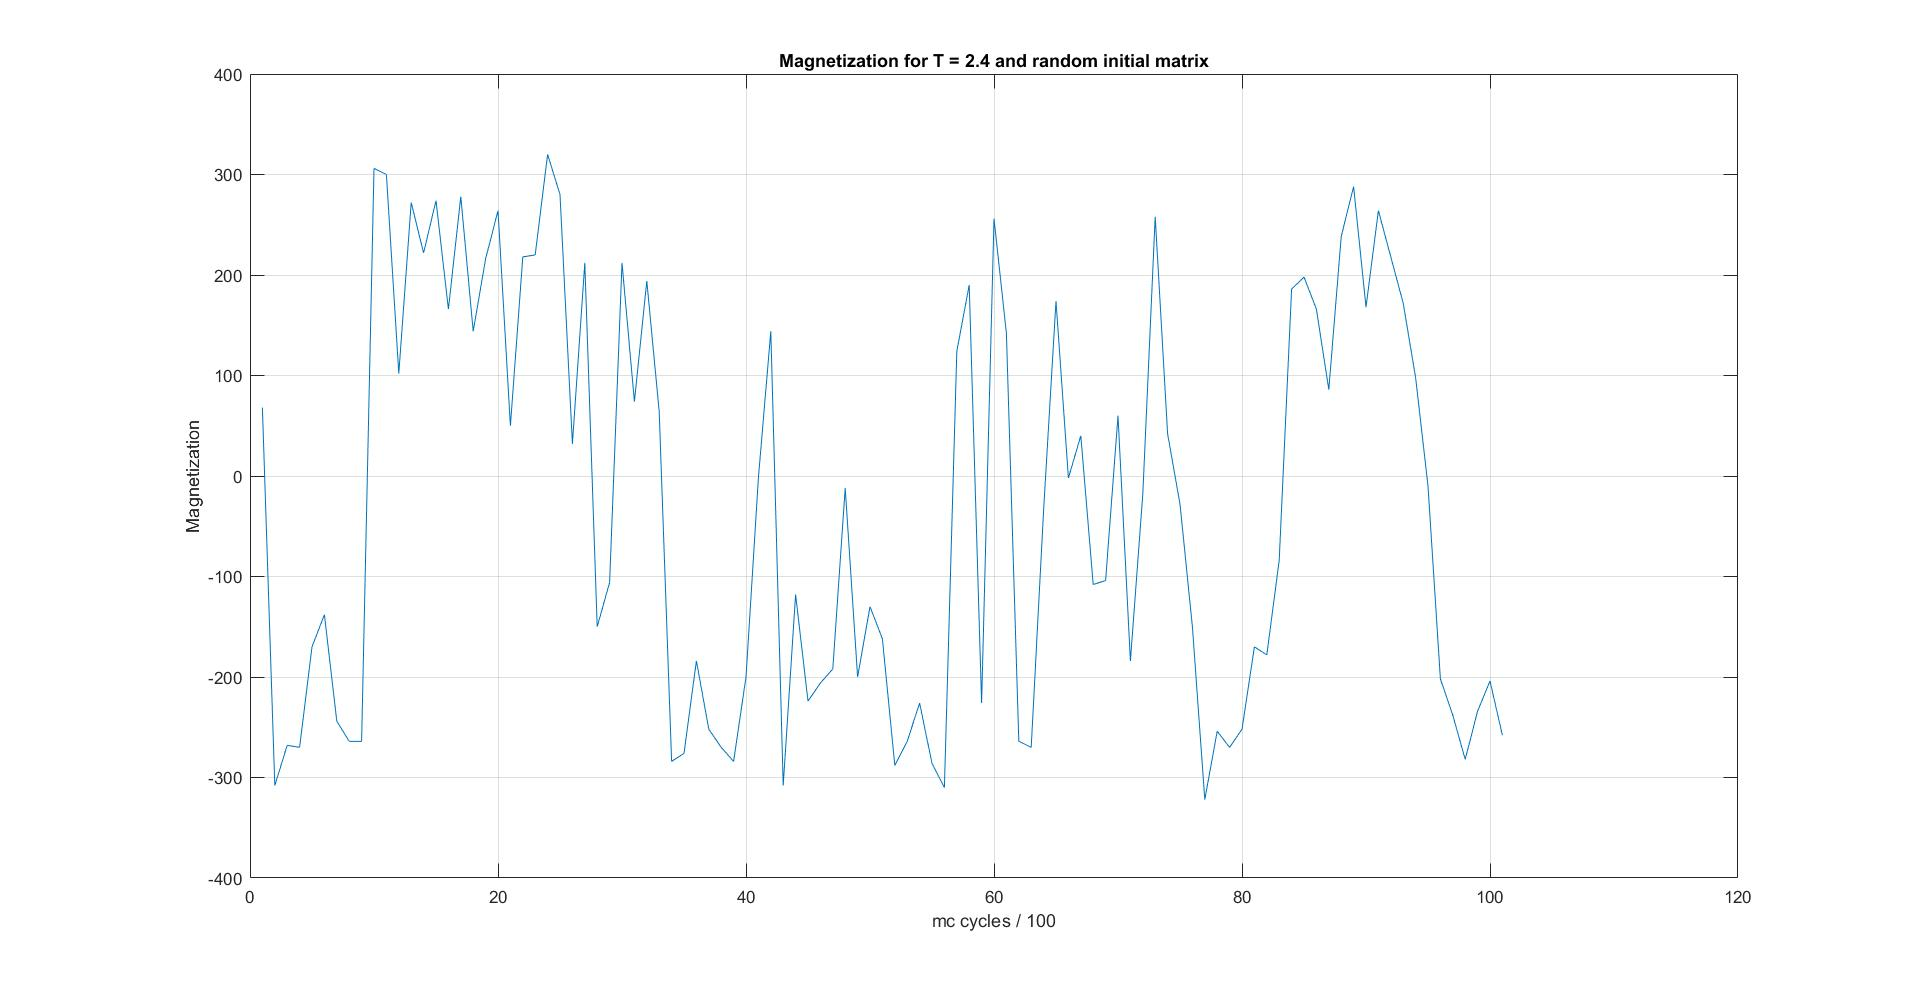
\includegraphics[scale=0.15]{magnetizationT24random}
}
\caption{Mean magnetization vs. Monte Carlo cycles for random oriented matrix with T=1.0 and T=2.4, respectively}
\label{fig:meanmagnran}
\end{figure}

\begin{figure}[H]
\centerline{
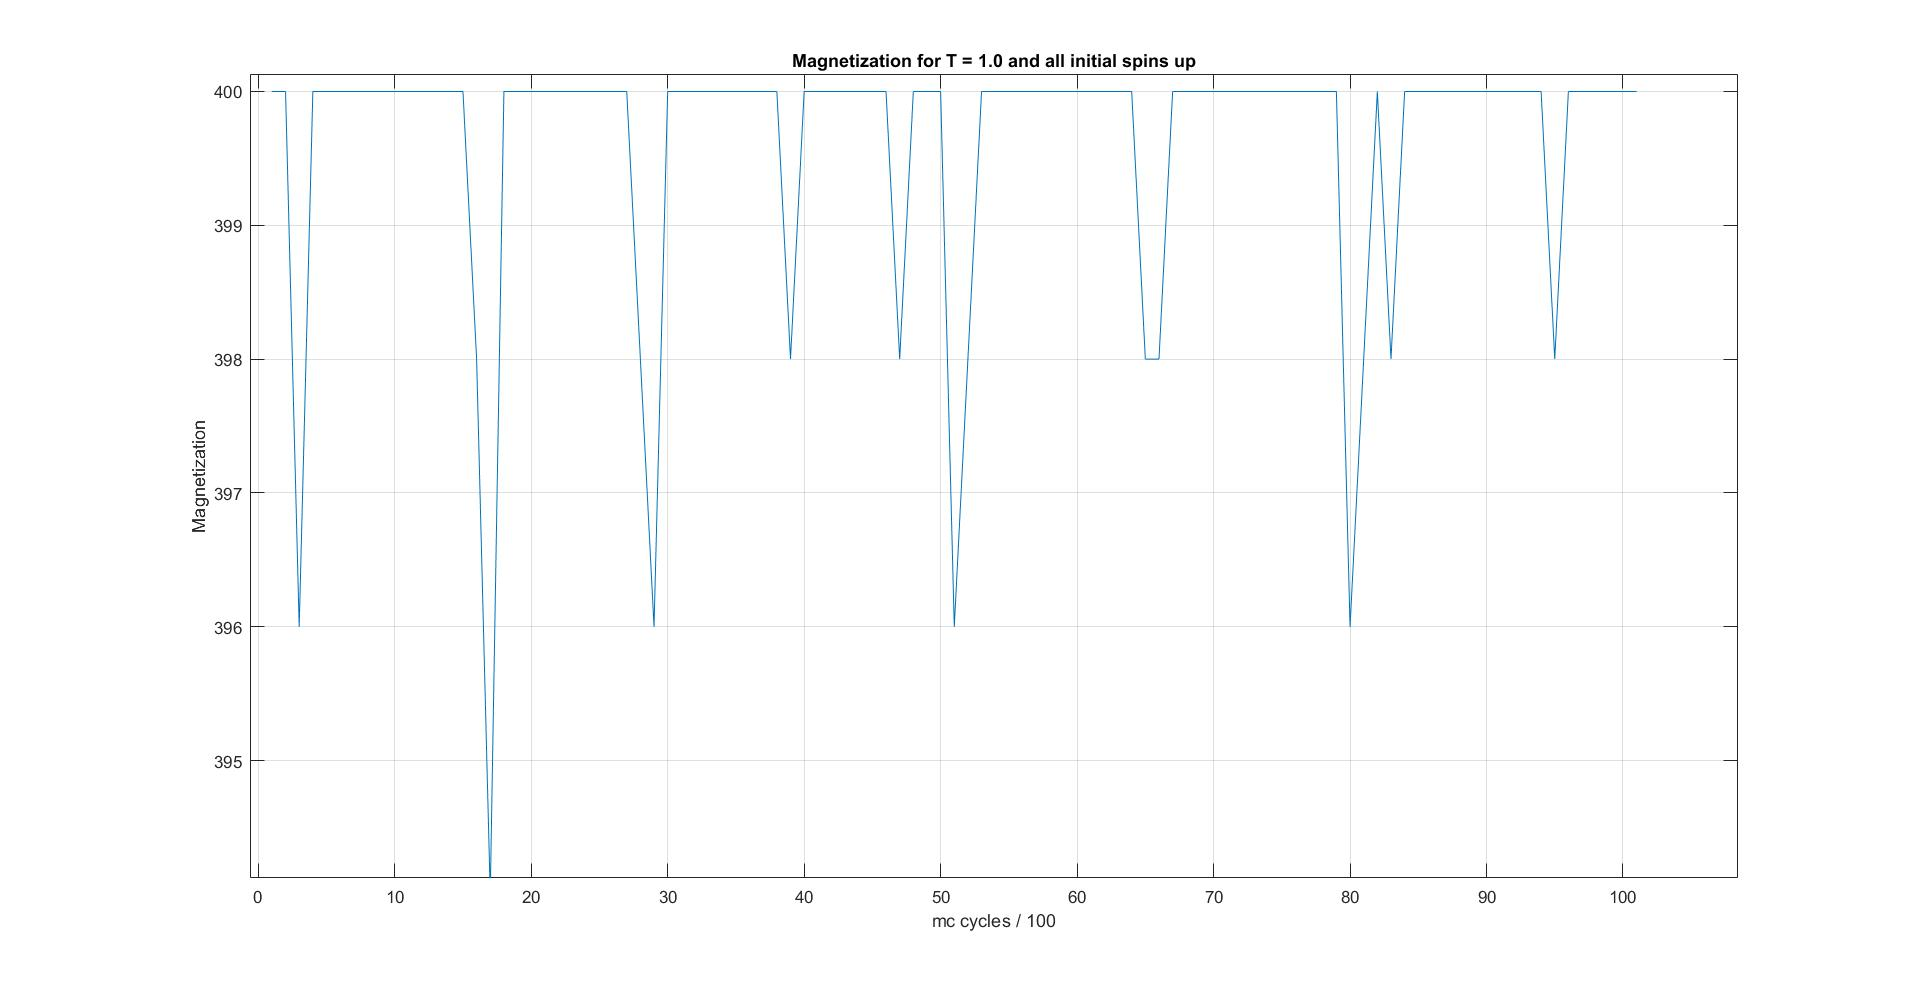
\includegraphics[scale=0.15]{magnetizationT1upspin}
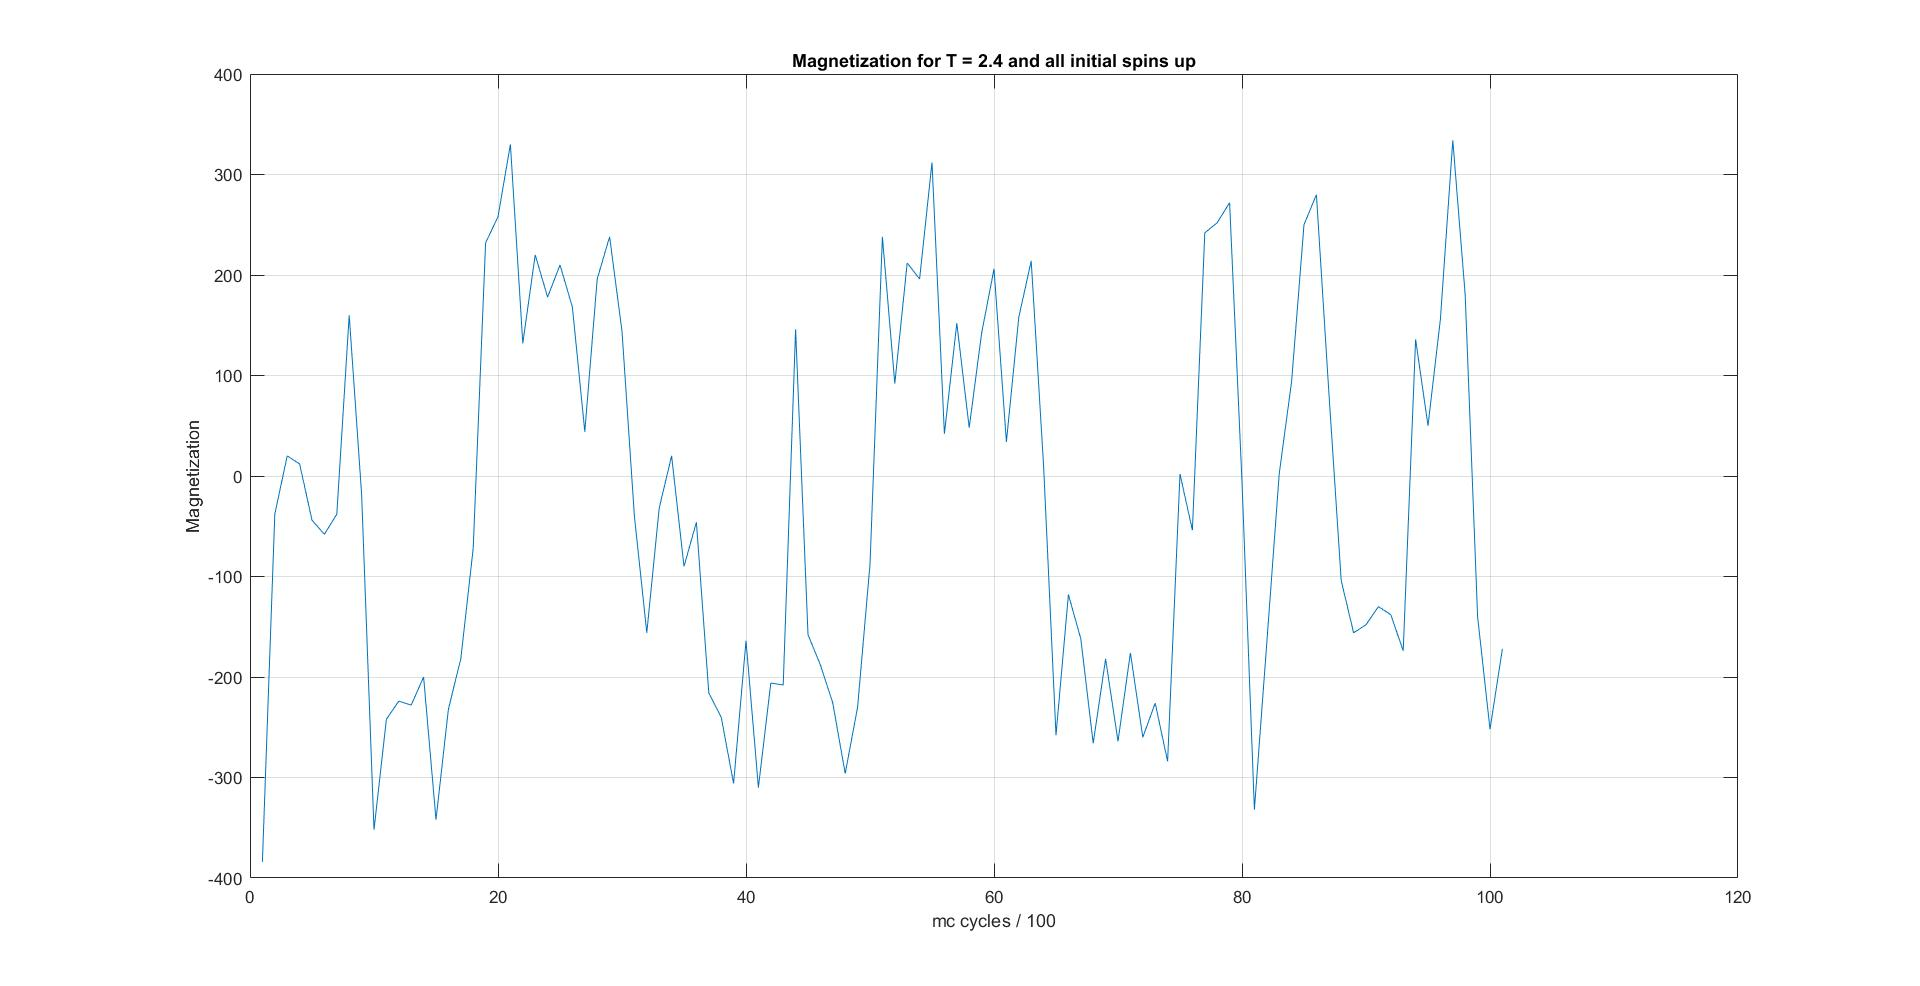
\includegraphics[scale=0.15]{magnetizationT24upspin}
}
\caption{Mean magnetization vs. Monte Carlo cycles for up-spin oriented matrix with T=1.0 and T=2.4, respectively}
\label{fig:meanmagnup}
\end{figure}

\noindent In figure \ref{fig:absmagn} it is noticeable that the absolute magnetization converges rapidly after the same amount of Monte Carlo cycles as the energy previously mentioned. The absolute magnetization behaves differently than the energy from figure \ref{fig:energy}, indicating that there are multiple lattice configurations giving the same energy minimum. (abs vs mean different??).
In figure \ref{fig:meanmagnran} and figure \ref{fig:meanmagnup} we notice that the magnetization oscillates between positive and negative values. Comparing this with figure \ref{fig:energy} and \ref{fig:absmagn}, it is noticeable that the magnetization keeps oscillating between positive and negative values after the energy and absolute magnetization has reached equilibrium.\\


\begin{figure}[H]
\centerline{
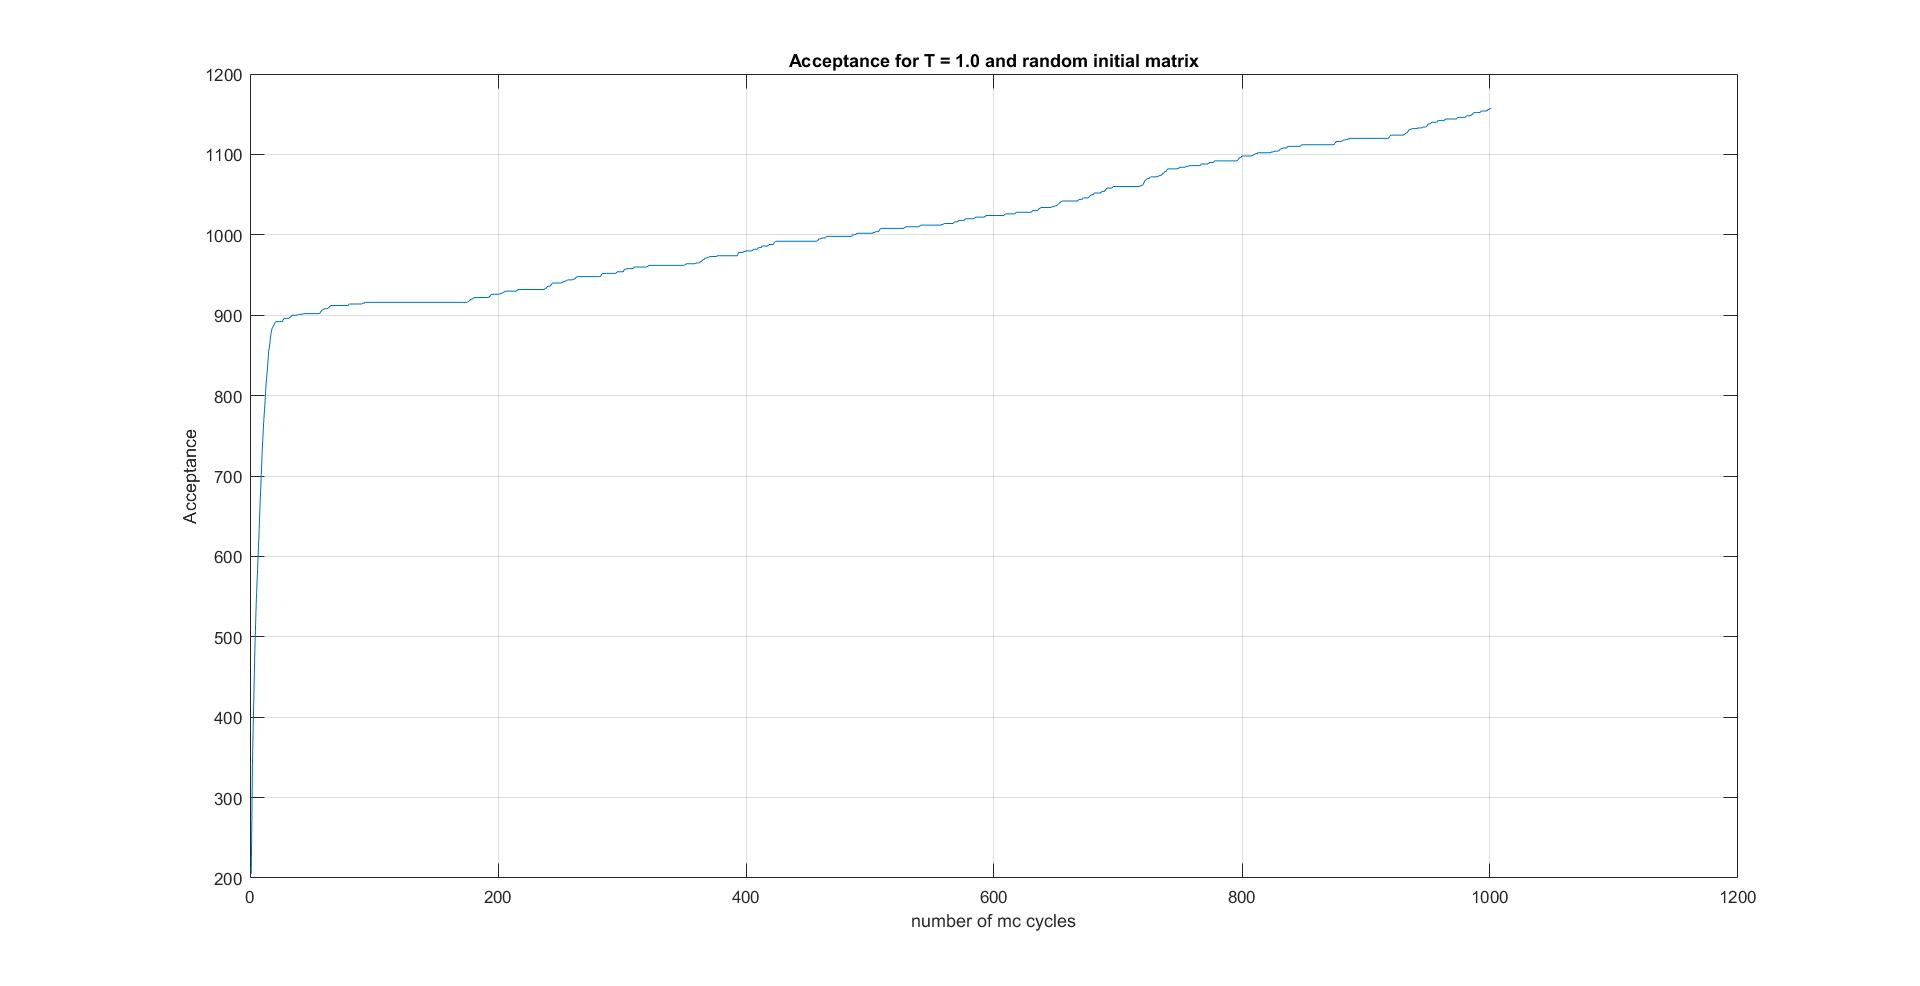
\includegraphics[scale=0.15]{acceptanceMCT1random}
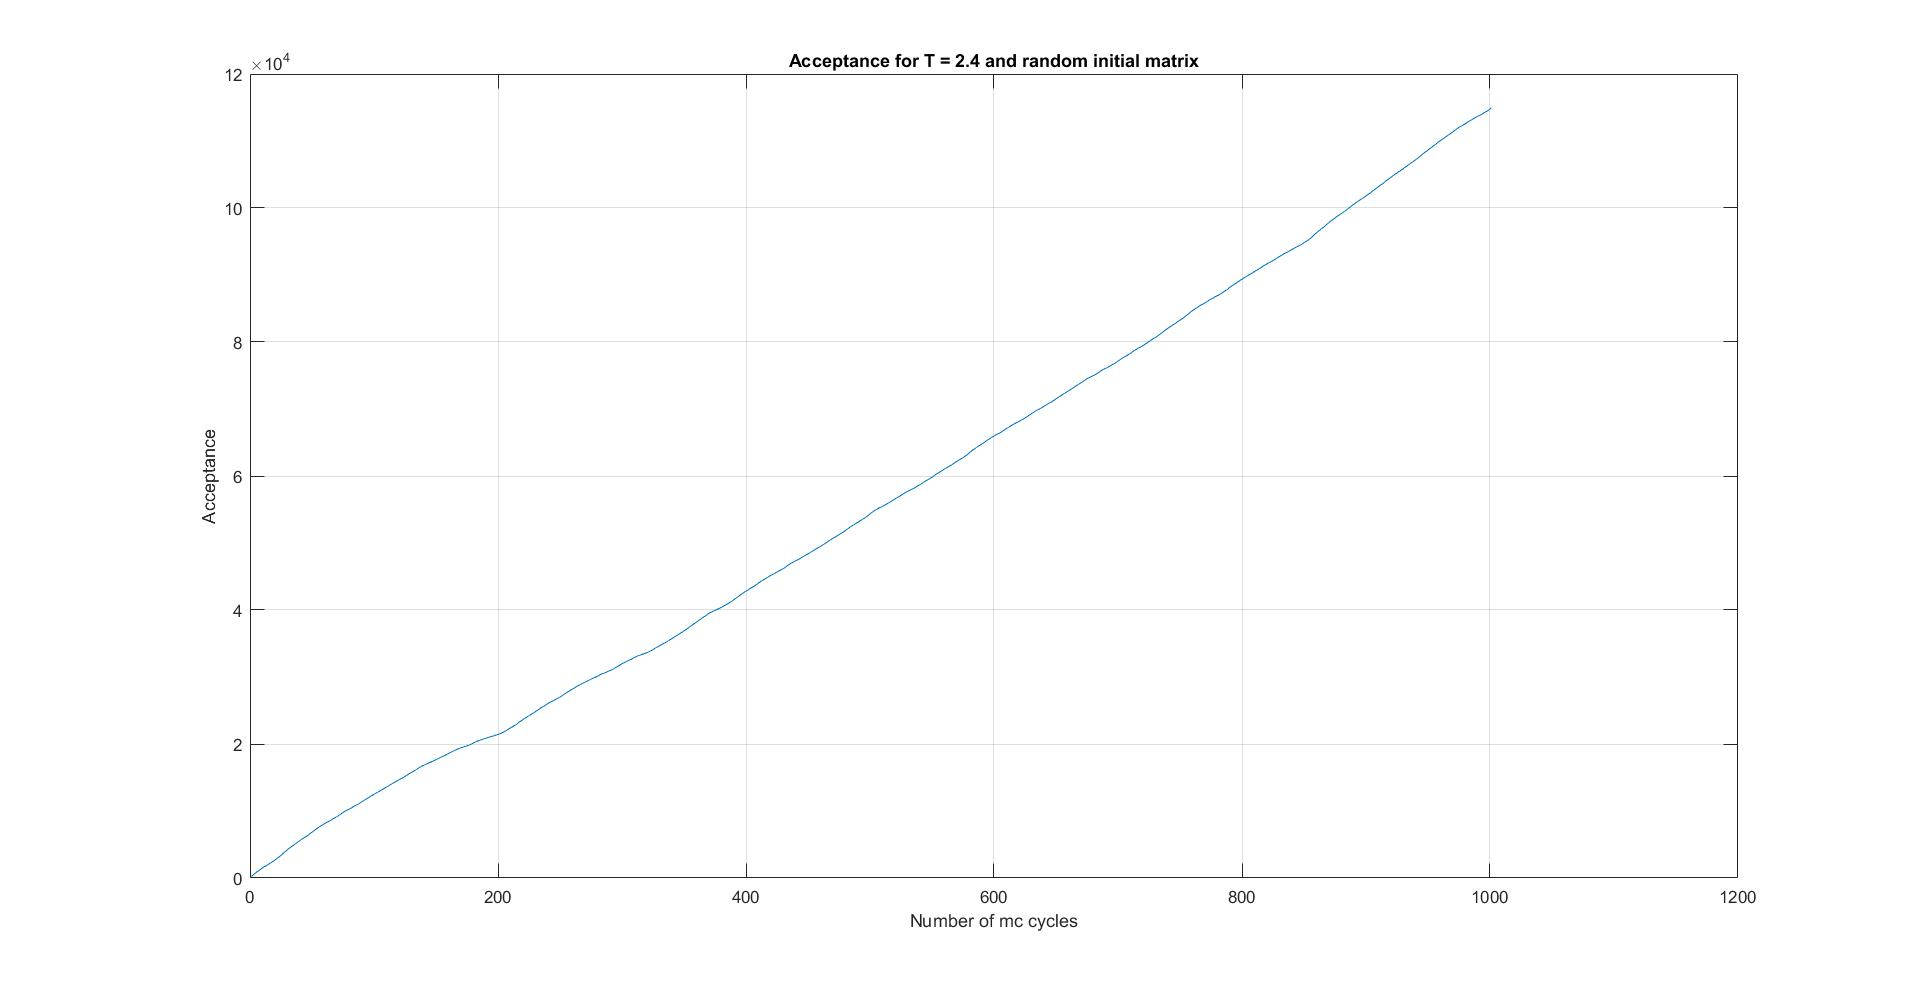
\includegraphics[scale=0.15]{acceptanceMCT24random}
}
\caption{Acceptance vs. Monte Carlo cycles for random oriented matrix with T=1.0 and T=2.4, respectively}
\label{fig:accran}
\end{figure}

\begin{figure}[H]
\centerline{
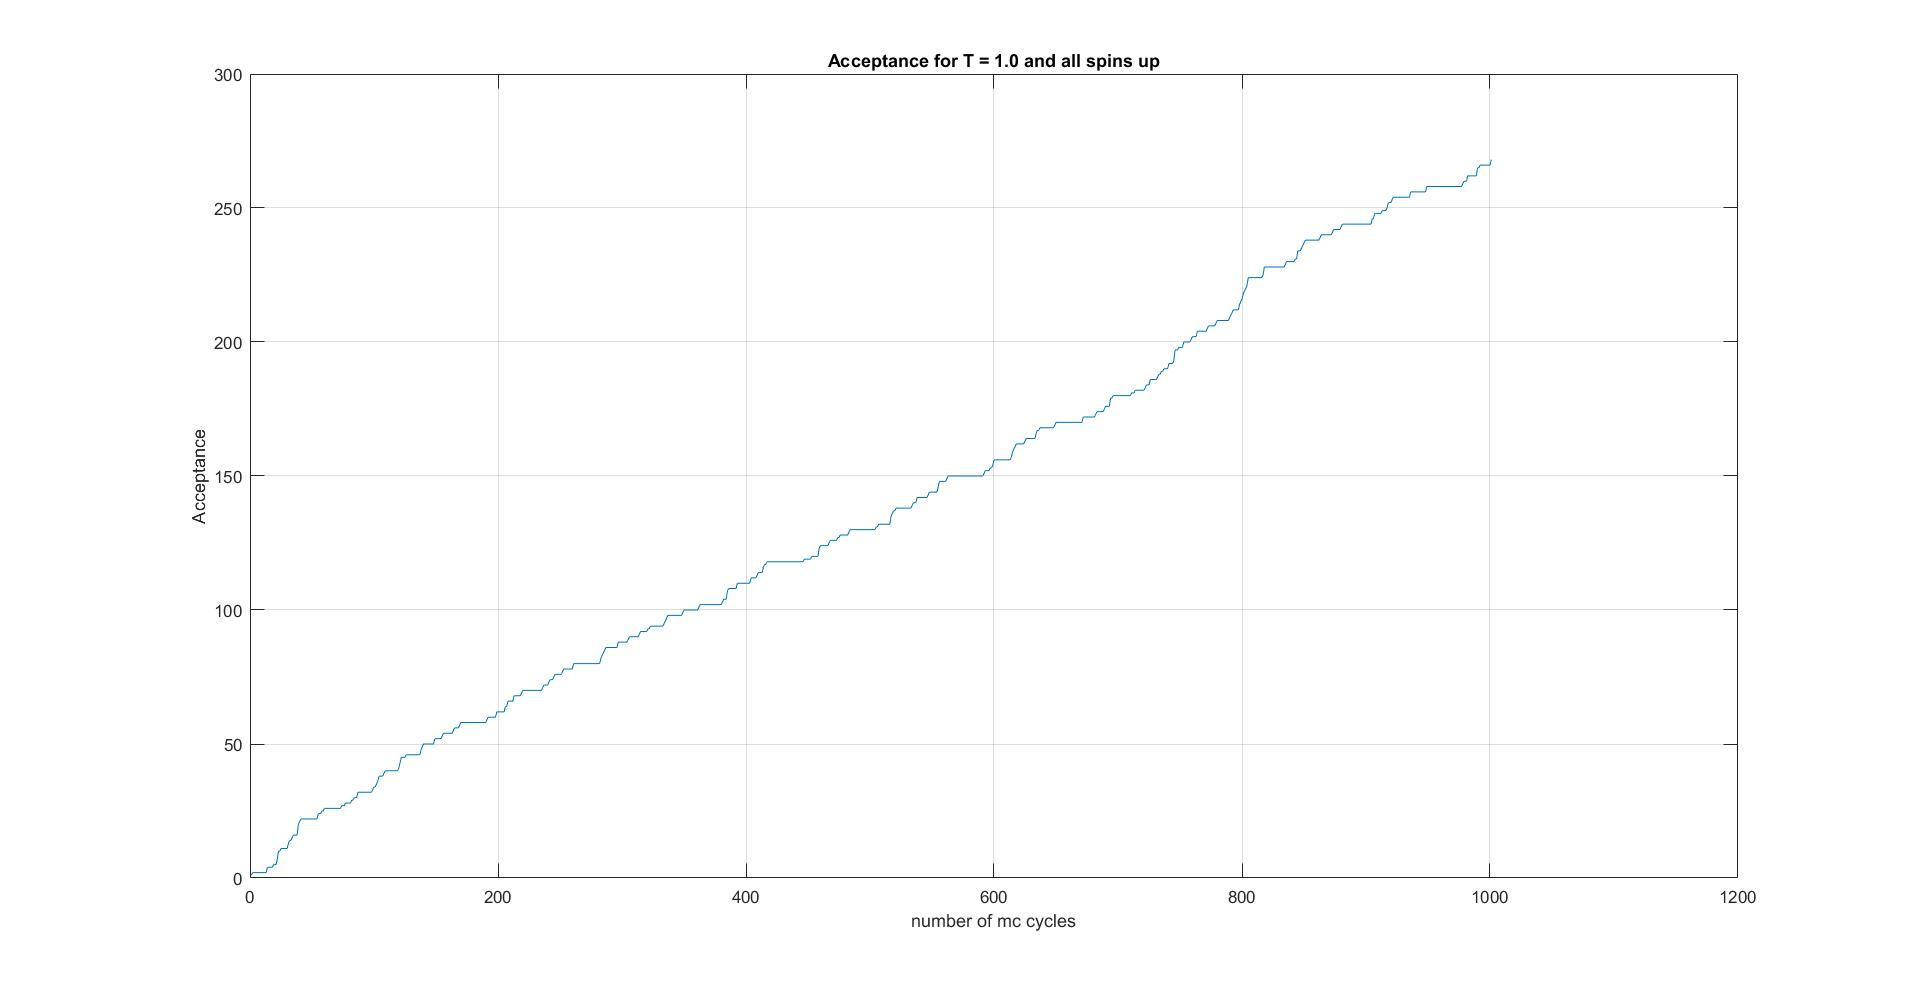
\includegraphics[scale=0.15]{acceptanceMCT1upspin}
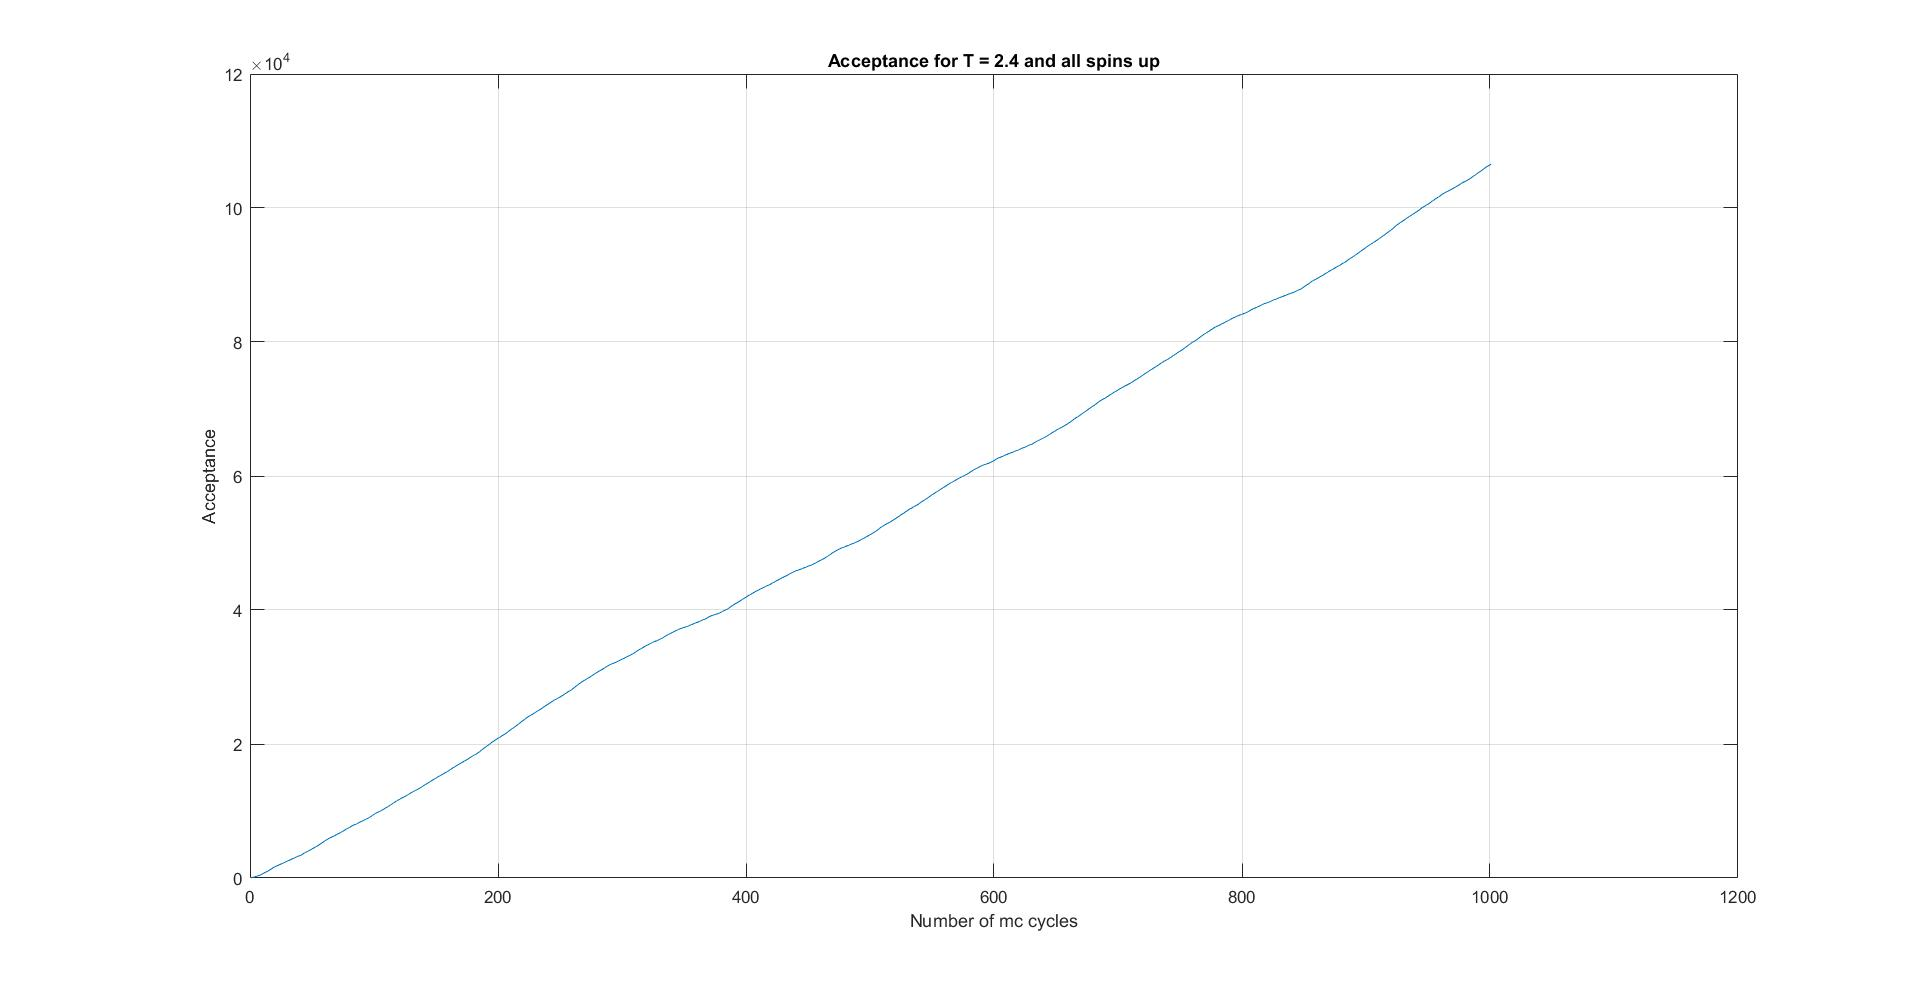
\includegraphics[scale=0.15]{acceptanceMCT24upspin}
}
\caption{Acceptance vs. Monte Carlo cycles for up-spin oriented matrix with T=1.0 and T=2.4, respectively}
\label{fig:accup}
\end{figure}

\begin{figure}[H]
\centerline{
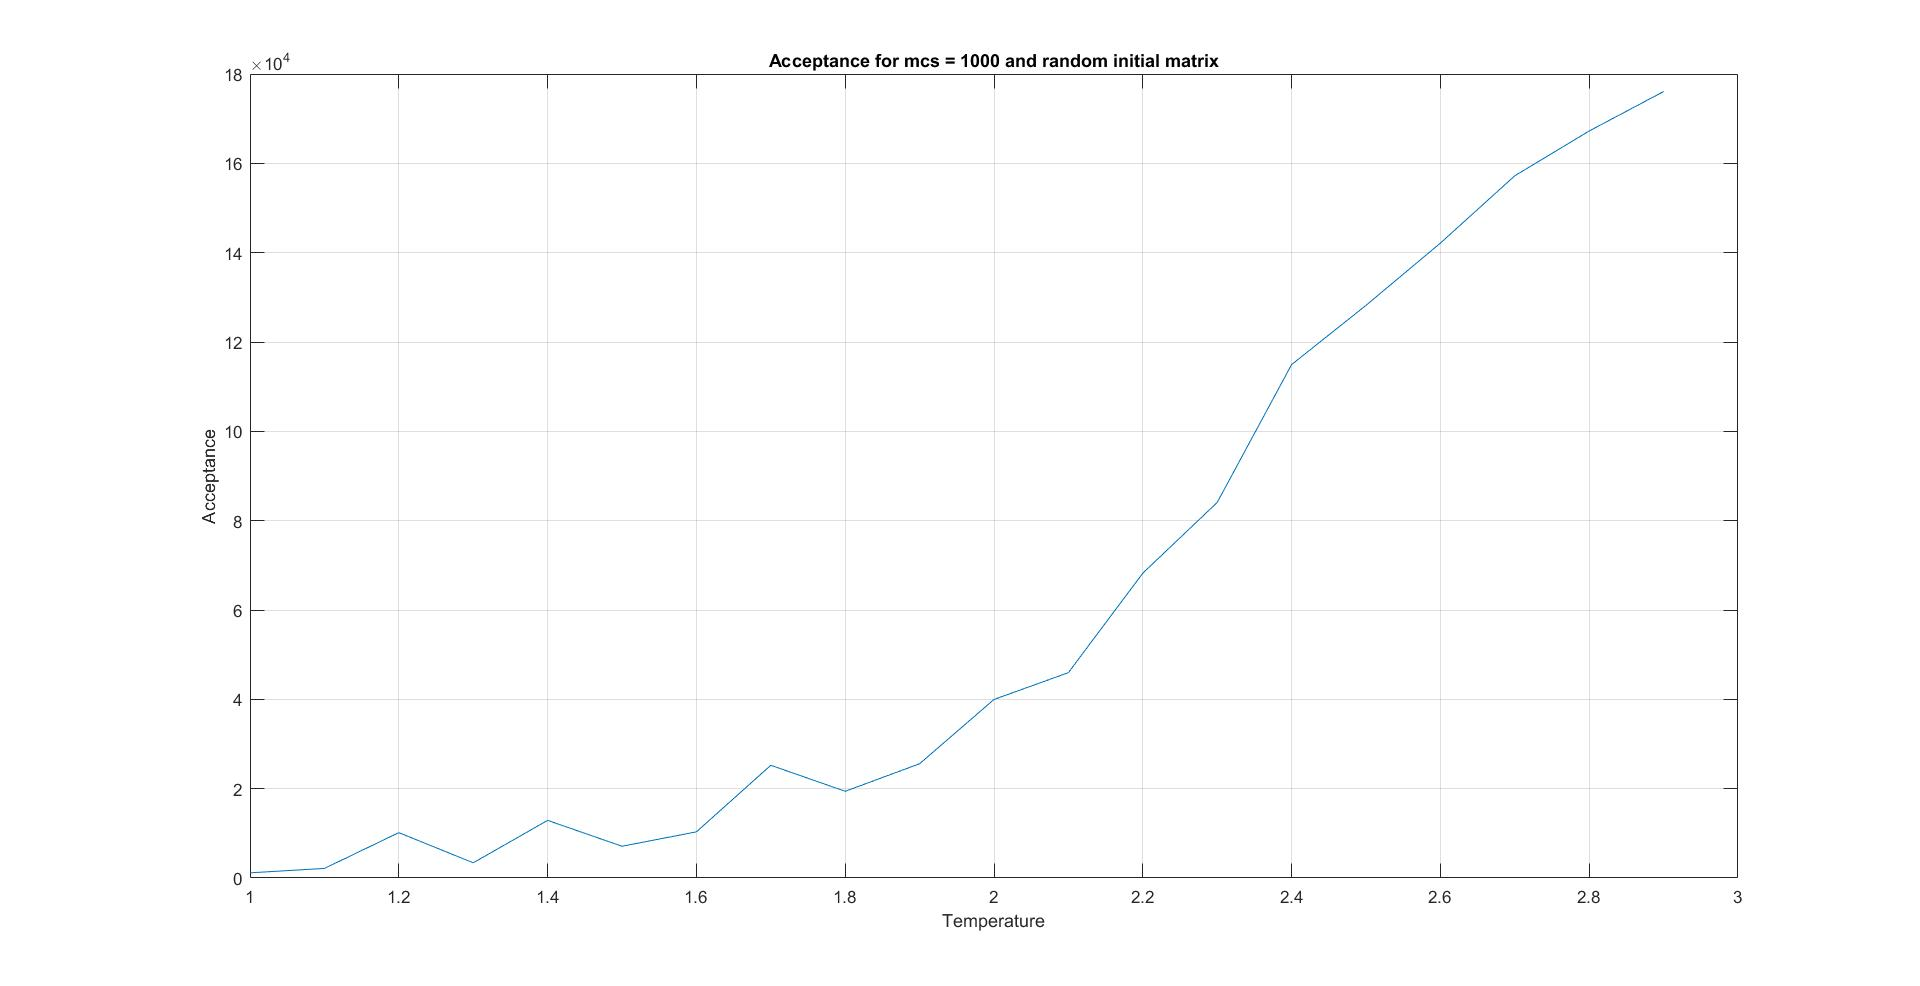
\includegraphics[scale=0.15]{acceptanceVStrandom}
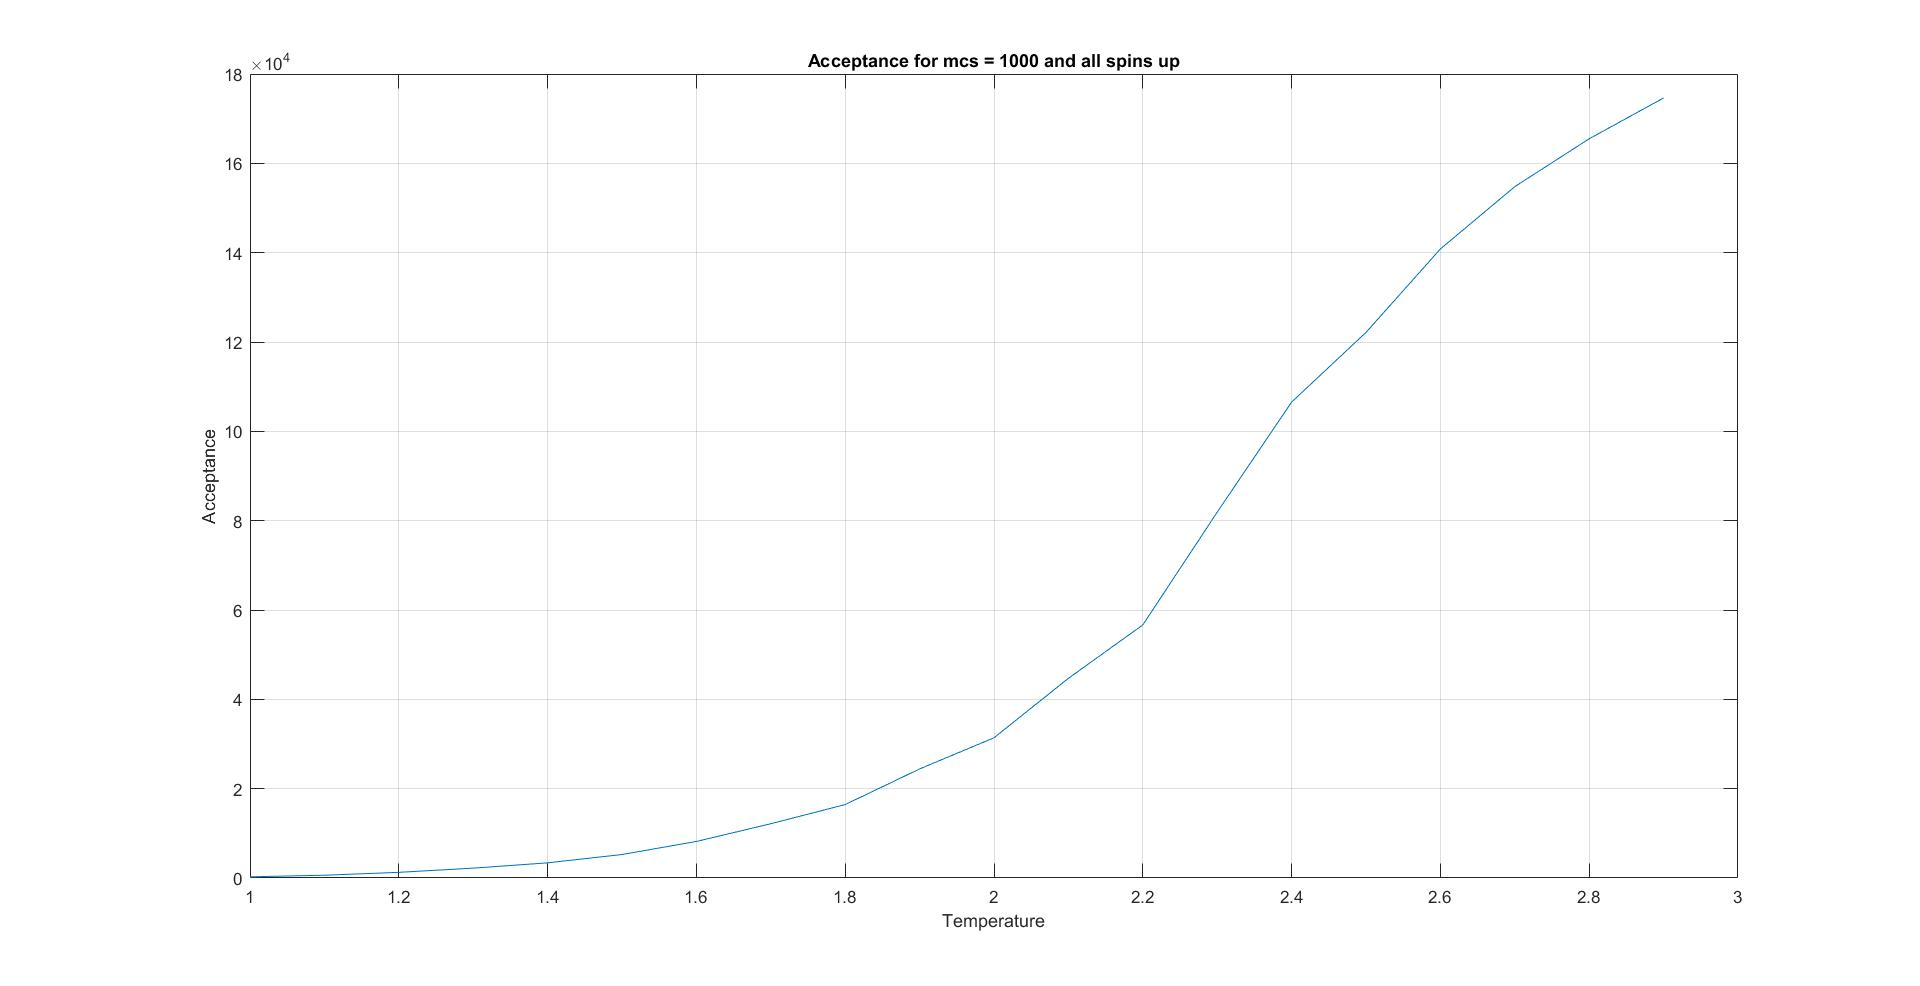
\includegraphics[scale=0.15]{acceptanceVStupspin}
}
\caption{Acceptance vs. temperature for random- and up-spin oriented matrix, respectively}
\label{fig:acctemp}
\end{figure}

\noindent For a random initial matrix and T=1, seen in figure \ref{fig:accran}, the system start off by accepting a lot of flips before behaving linearly as the initial up-spin matrix with T=1, shown in figure \ref{fig:accup}. This is because the random intial matrix does not start at the equilibrium. For T=2.4 there are a lot more accepted configurations. None of the matrices start at equilibrium and seem to behave the same.\\
In figure \ref{fig:acctemp} we can clearly see an exponential growth in number of accepted configurations for increasing temperature. It seem like the number of accepted configurations might converge at the end of the graph, but we would need to run for higher temperatures to be sure about this. The up-spin initial matrix is smoother than the random initial matrix, which is expected.\\


\begin{figure}[H]
\centerline{
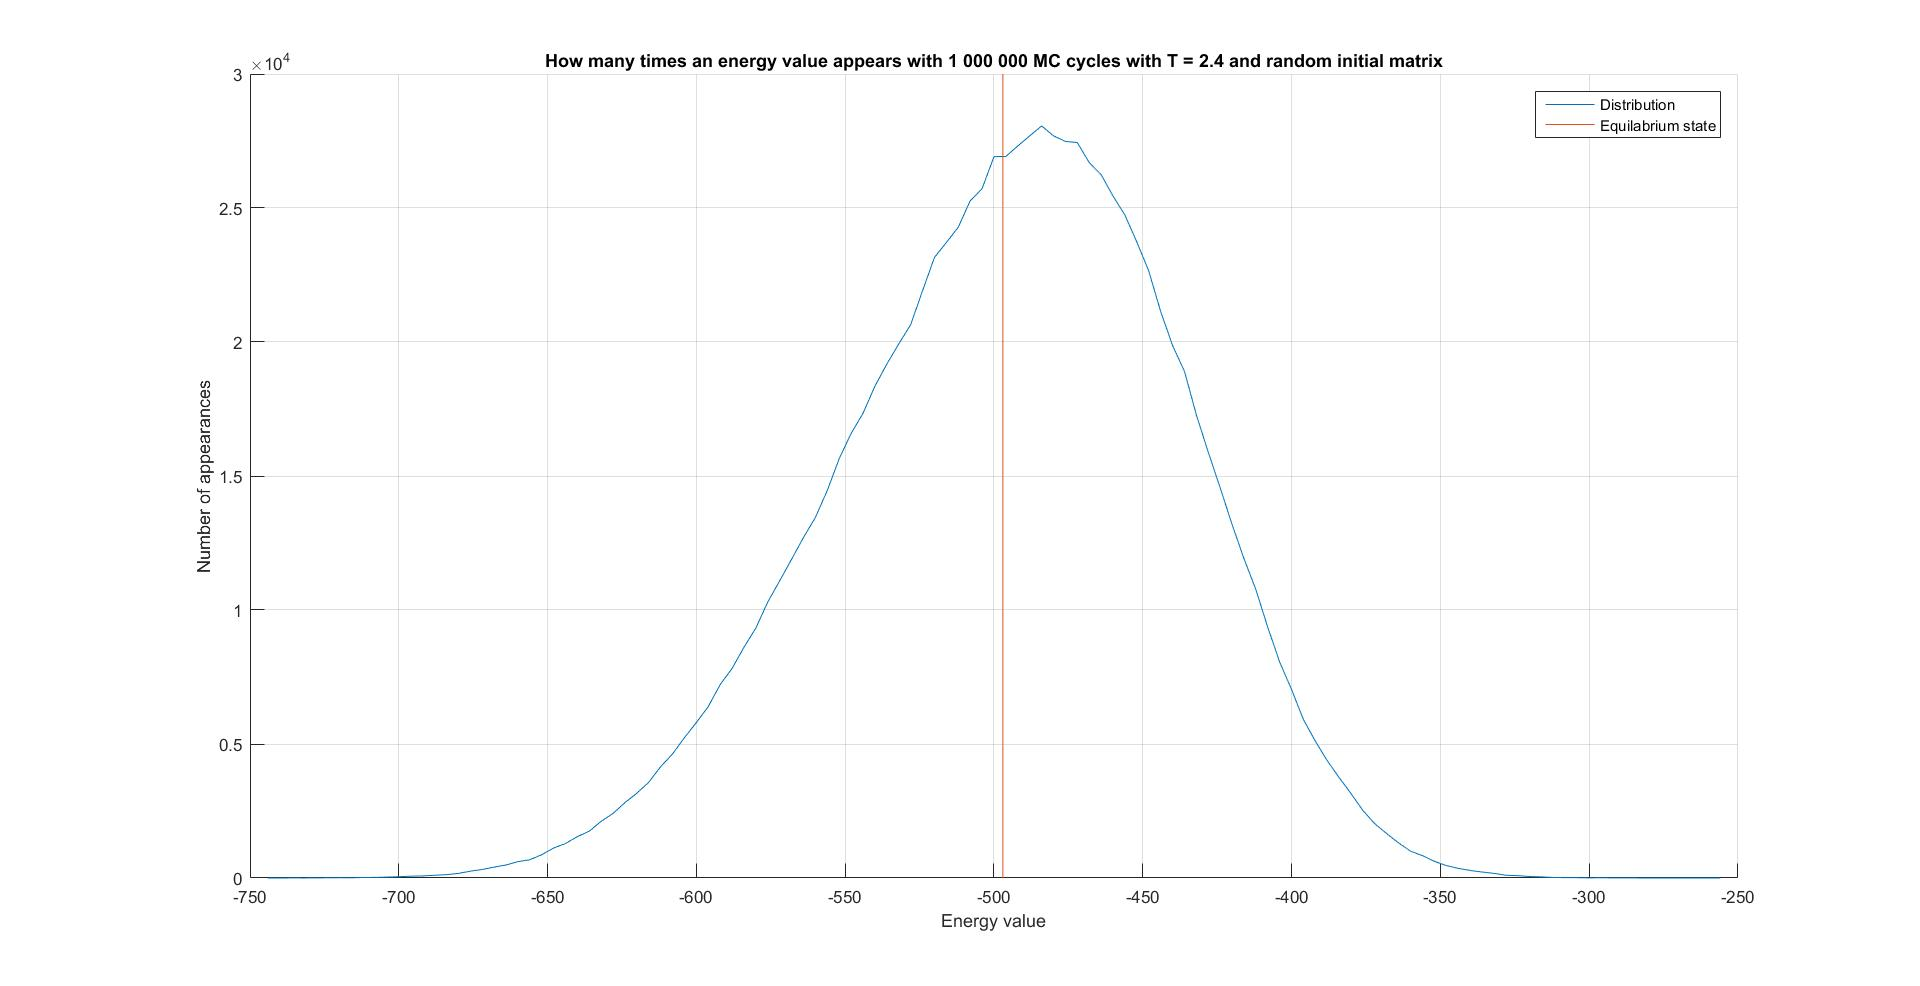
\includegraphics[scale=0.15]{energyappearanceT24random}
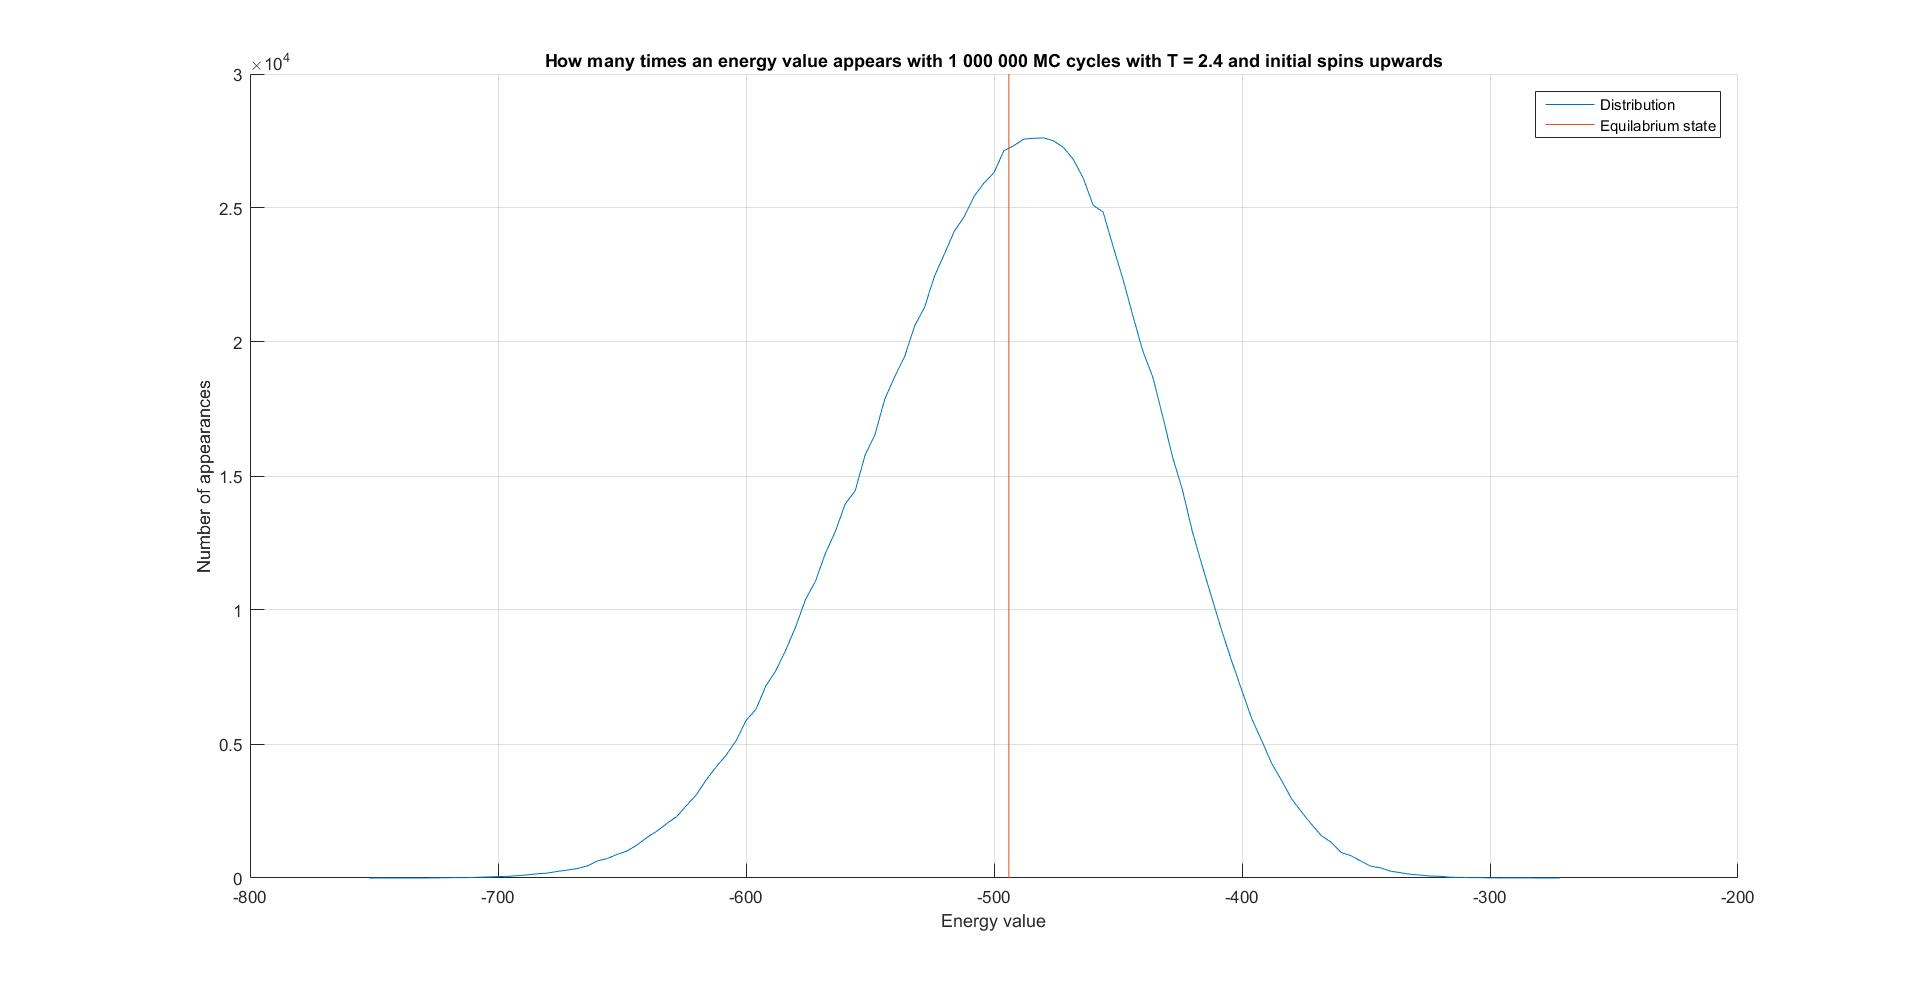
\includegraphics[scale=0.15]{energyappearanceT24upspin}
}
\caption{Number of appearances per energy value for random- and up-spin oriented matrix with T=2.4}
\label{fig:dist}
\end{figure}

\begin{figure}[H]
\centerline{
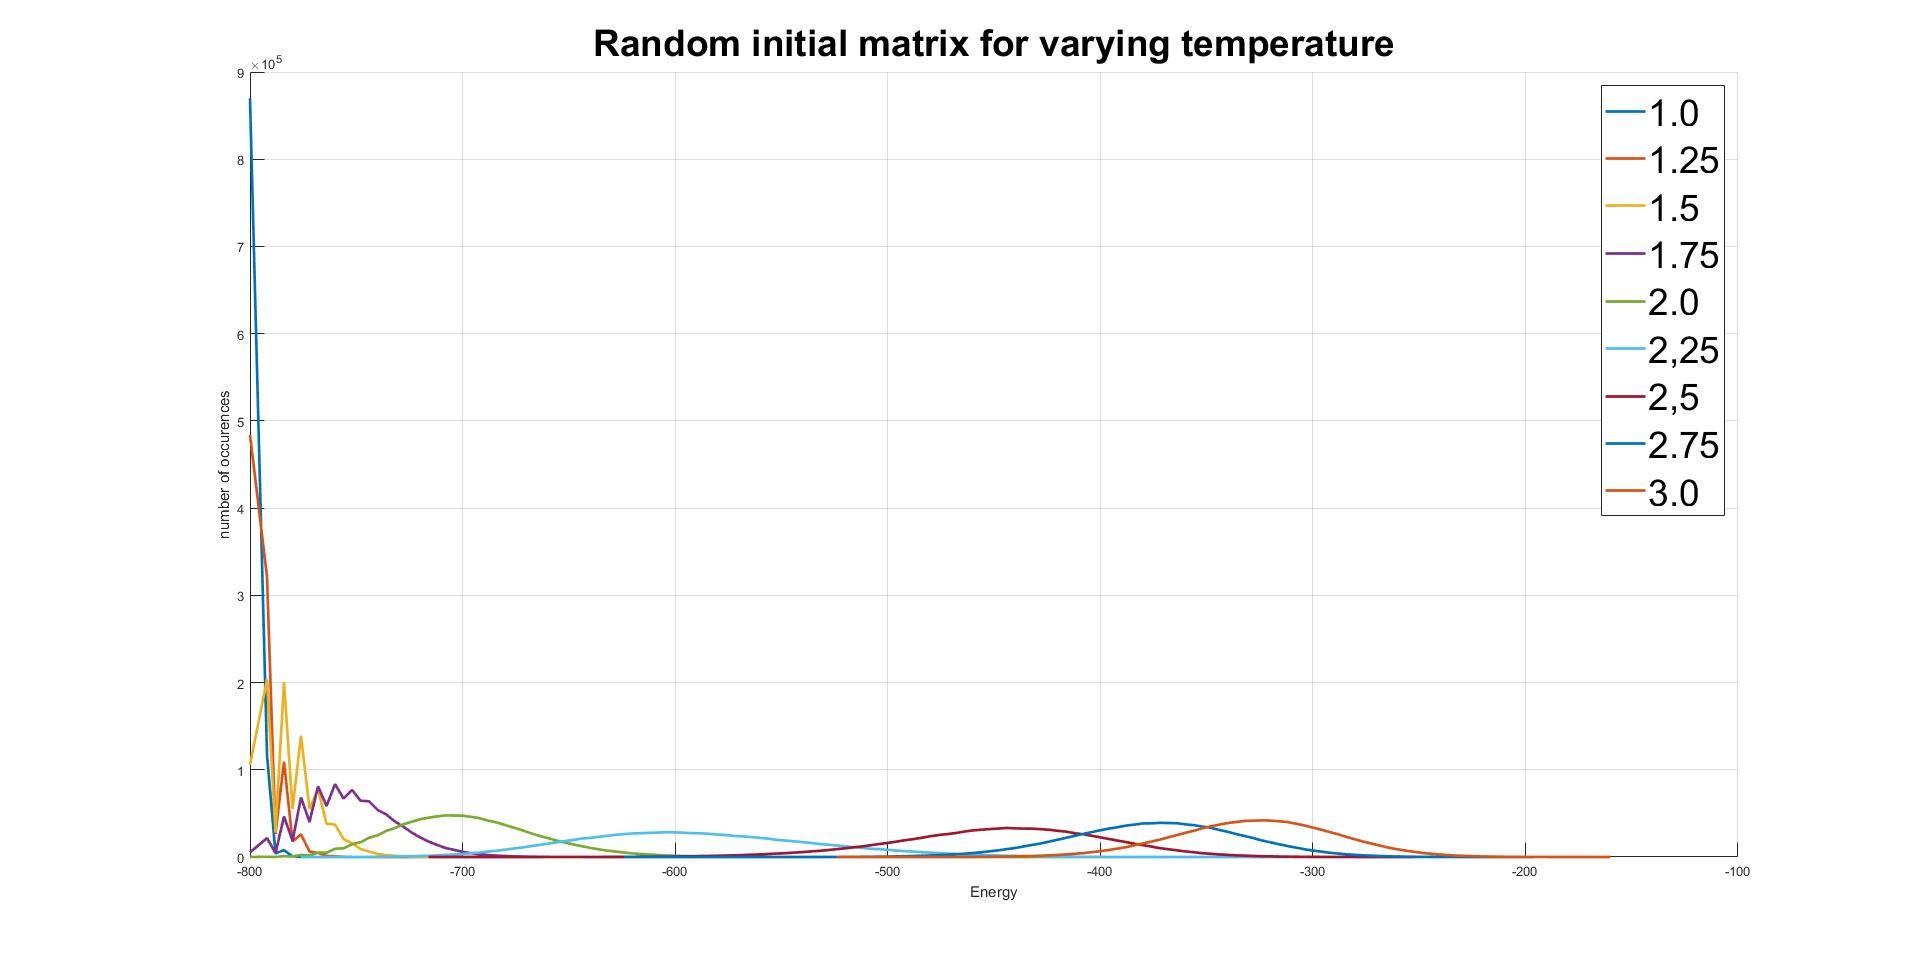
\includegraphics[scale=0.3]{energyapperanceTvarRan}
}
\caption{Probability distribution for varying temperature over $10^6$ Monte Carlo cycles}
\label{fig:distvar}
\end{figure}



\begin{center}
\begin{table} [H]
\caption{Variance in energy for different temperatures over $10^6$ Monte Carlo cycles} \label{tab:table3}
\centerline{
\begin{tabular}{c|c}
Temperature& Variance\\
1.00&0.0227441\\
1.25&0.129337\\
1.50&0.444368\\
1.75&1.18547\\
2.00&2.88226\\
2.25&7.89626\\
2.50&6.18416\\
2.75&4.25249\\
3.00&3.61595\\
\end{tabular}
}
\end{table}
\end{center}

\noindent The probability distribution in figure \ref{fig:dist} show a negative skewed distribution, with the mean value laying one the left side of the mode. SUMSUM
From figure \ref{fig:distvar} we can clearly see that there are a higher probability for higher energies for increasing temperature. It is also noticeable that the energy is also oscillating more for higher temperatures. For T=1 there are almost only the equilibrium state. 
\\


\begin{figure}[H]
\centerline{
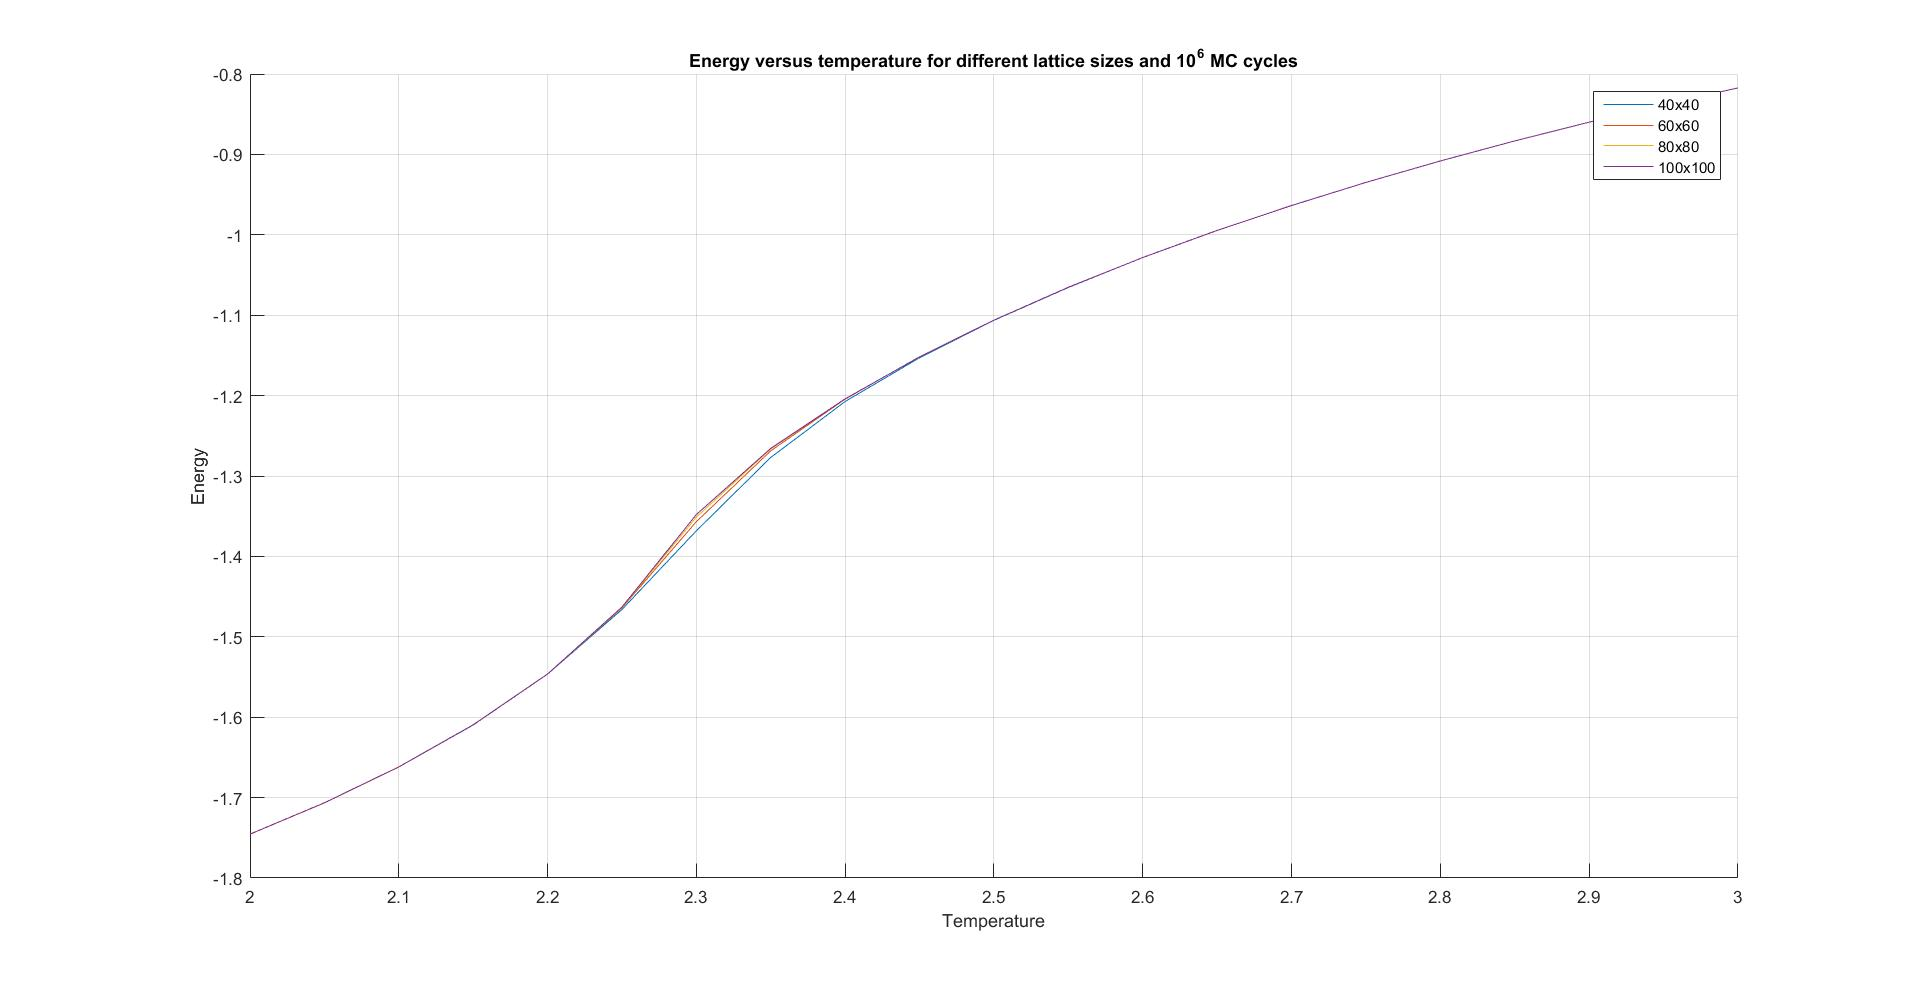
\includegraphics[scale=0.3]{energyVSt}
}
\caption{Mean energy vs. temperature for $10^6$ Monte Carlo cycles normalized(single lattice objects)}
\label{fig:energyL}
\end{figure}

\begin{figure}[H]
\centerline{
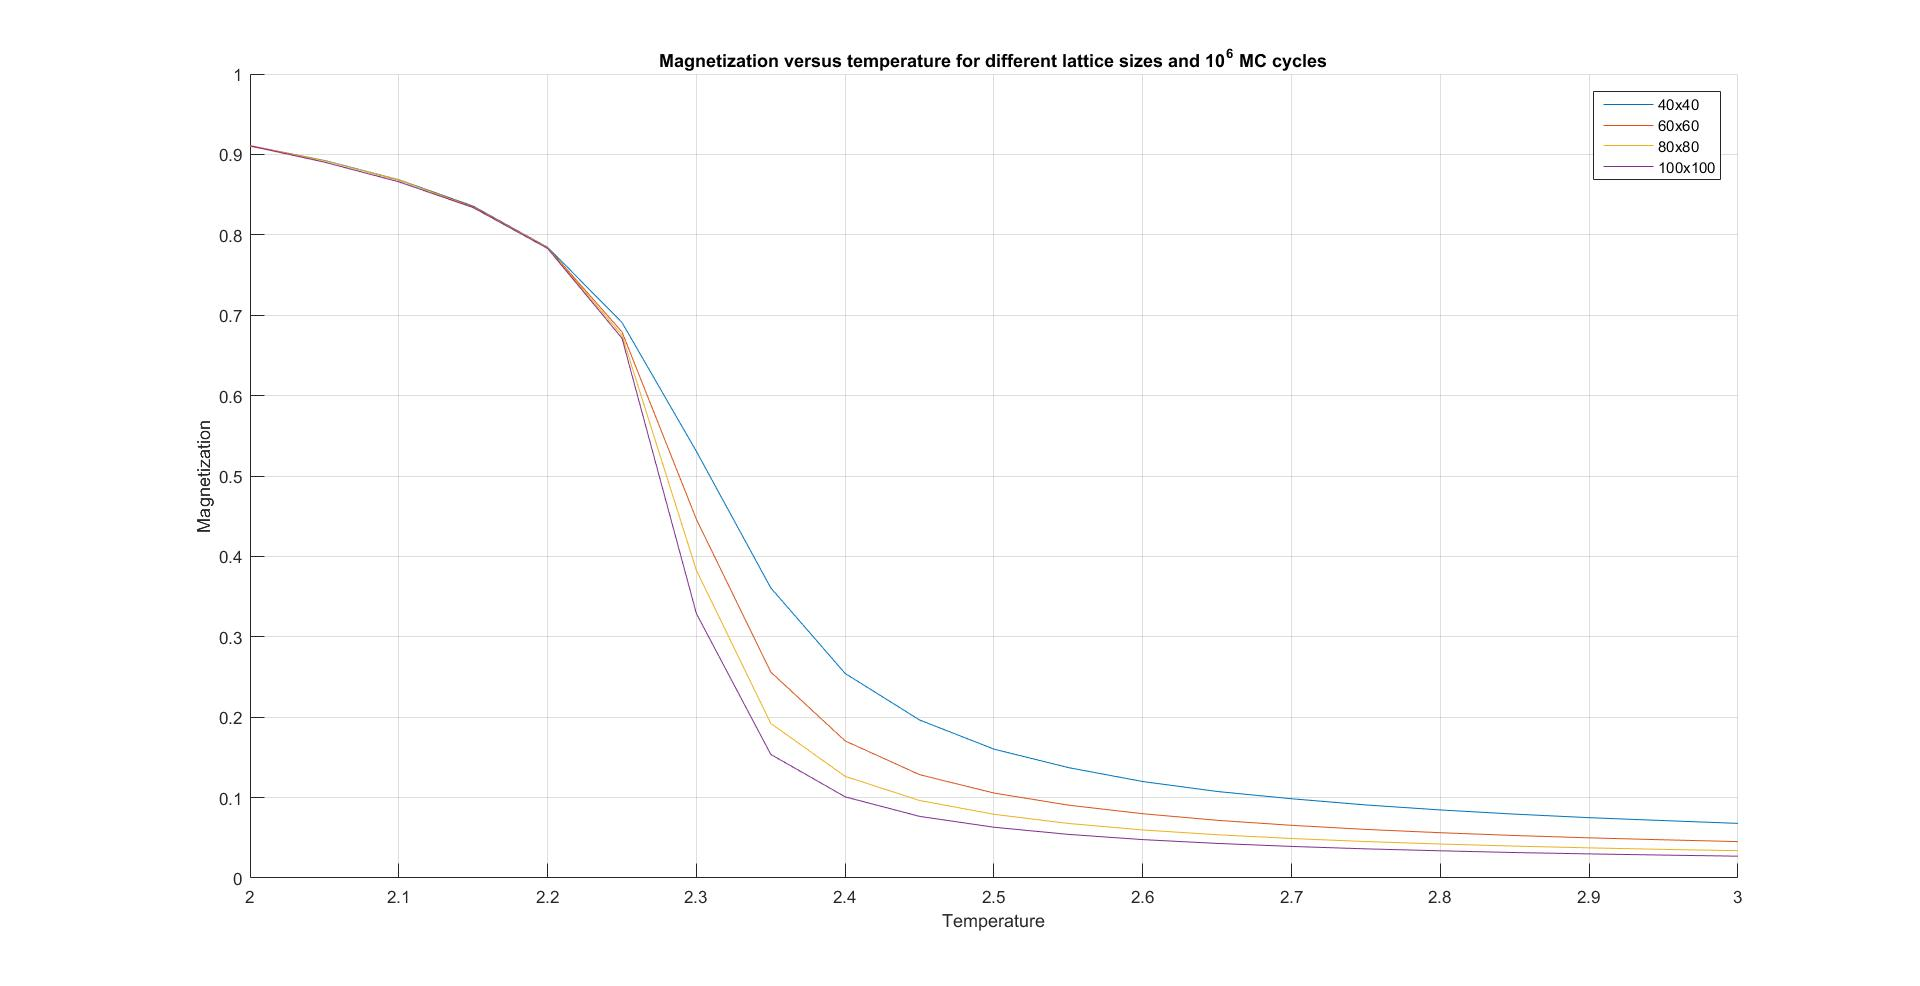
\includegraphics[scale=0.3]{magnetizationVSt}
}
\caption{Mean magnetization vs. temperature for $10^6$ Monte Carlo cycles normalized(single lattice objects)}
\label{fig:magnL}
\end{figure}

\begin{figure}[H]
\centerline{
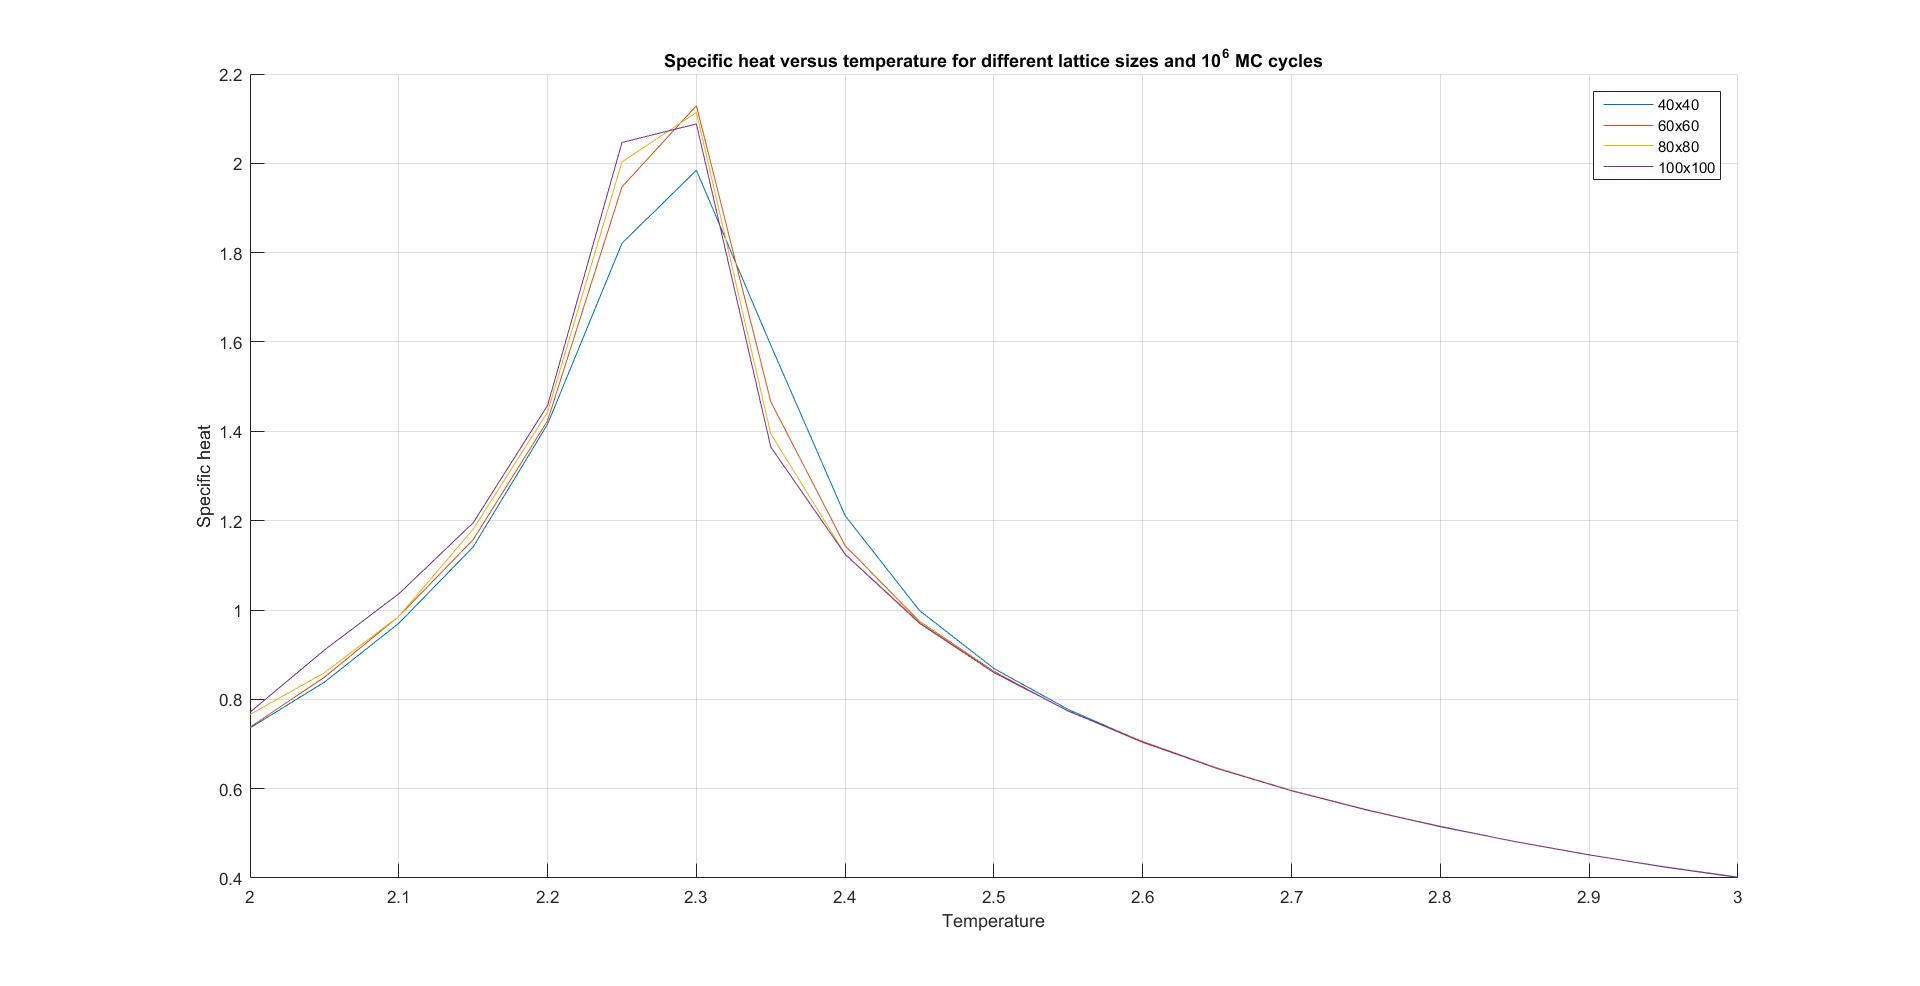
\includegraphics[scale=0.3]{heatVSt}
}
\caption{Specific heat vs. temperature for $10^6$ Monte Carlo cycles normalized(single lattice objects)}
\label{fig:heatL}
\end{figure}

\begin{figure}[H]
\centerline{
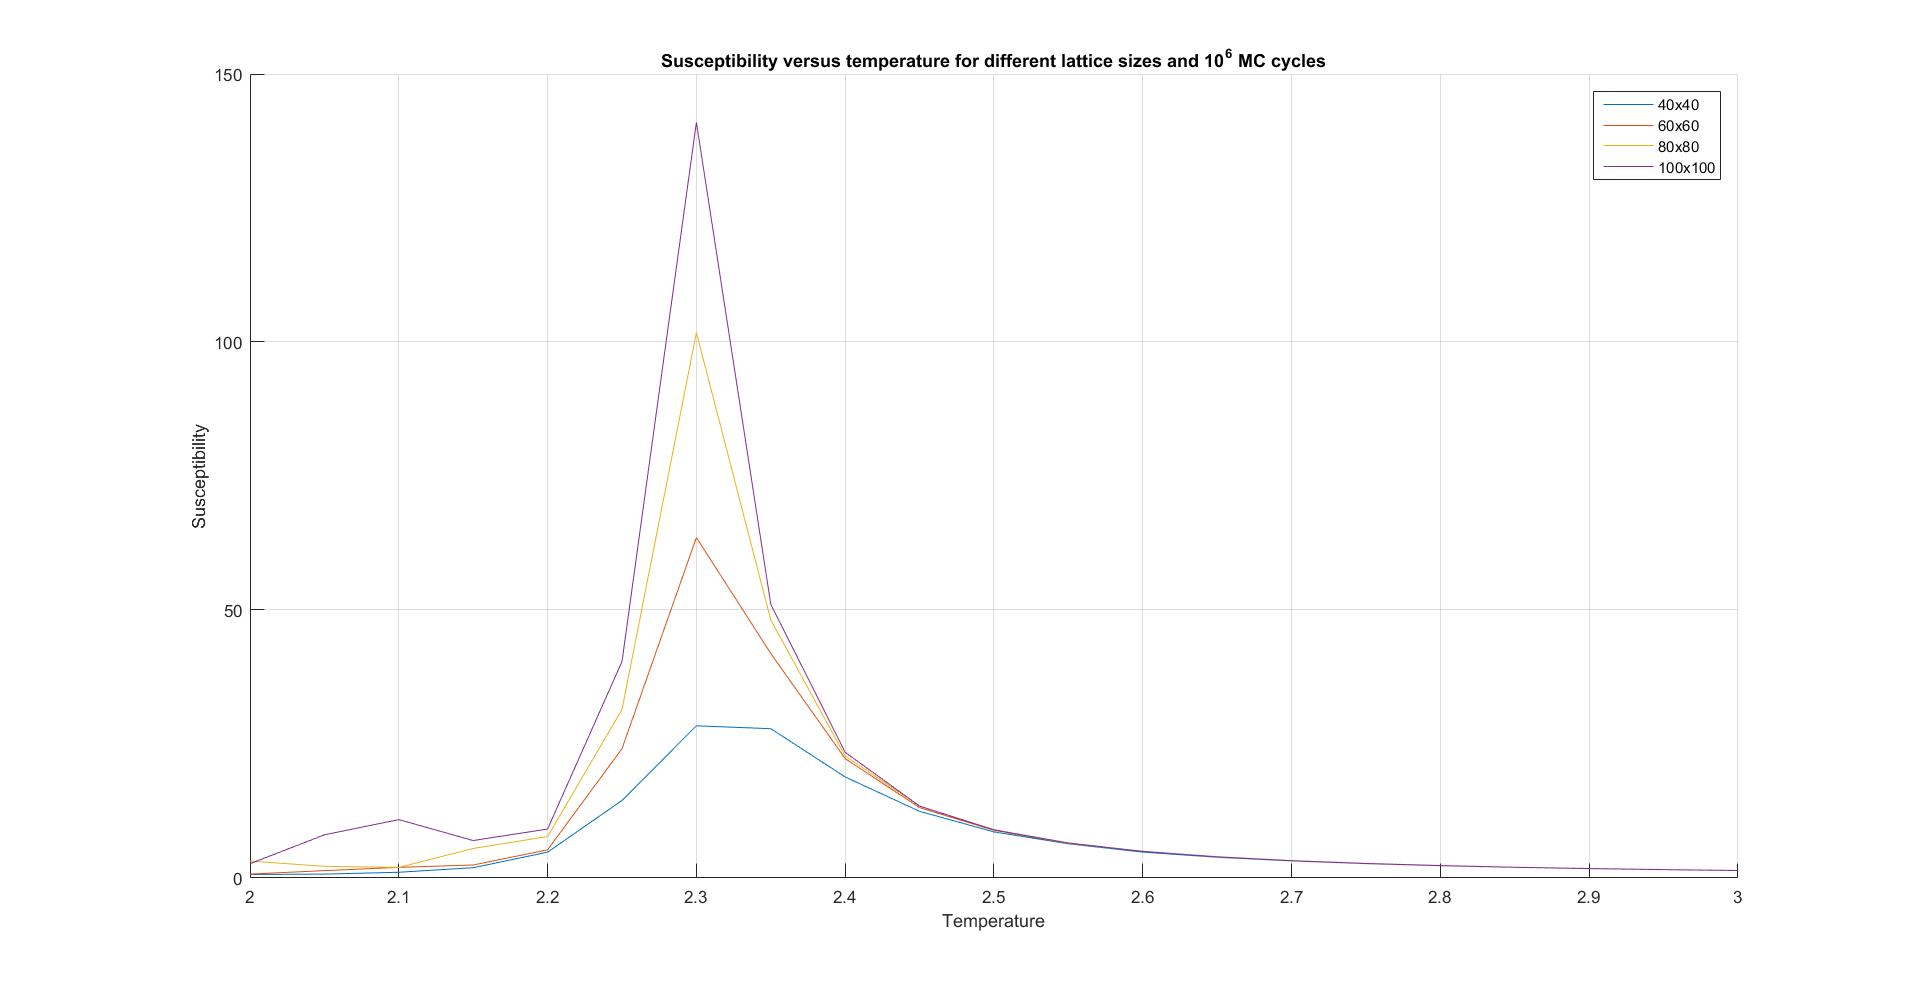
\includegraphics[scale=0.3]{susceptibilityVSt}
}
\caption{Susceptibility vs. temperature for $10^6$ Monte Carlo cycles normalized(single lattice objects)}
\label{fig:susL}
\end{figure}

\begin{center}
\begin{table} [H]
\caption{Run time for different lattice sizes with $10^6$ MC cycles} \label{tab:table4}
\centerline{
\begin{tabular}{c|c}
Lattice size& Time in seconds\\
60x60 & 3996.57\\
80x80 & 7081.15\\
100x100 & 18630.9\\
\end{tabular}
}
\end{table}
\end{center}

\noindent The critical temperature seem to be the same value of 2.3, for all matrices, looking at both the specific heat and the susceptibility in figure \ref{fig:heatL} and \ref{fig:susL}. This is disappointing as this of course will give us the same value of 2.3 for the critical temperature in the thermodynamic limit $L \rightarrow \infty$. Comparing this critical temperature with figure \ref{fig:energyL} and \ref{fig:magnL}, it seems that this value would be found as the double derivative of these functions.

\newpage
{\LARGE\bf
Discussion
}\\

\noindent For a 2x2 lattice the analytical and numerical solutions correlate well after few Monte Carlo cycles.\\
\noindent For T=2.4 the energy oscillate more than for T=1. This is expected as energy is more active at higher temperatures.\\
Looking at the different magnetization plots it is noticeable that the magnetization is limited to some set values. The reasoning for this is the same as for the 2x2 lattice having few possible configurations. In the same way as for the 2x2 lattice, a larger lattice will only have a set number of values it can jump between when doing leaps between positive and negative magnetization values. The reason for the mean magnetization to keep oscillating between positive and negative values, in figure \ref{fig:meanmagnran} and \ref{fig:meanmagnup} for T=2.4, after the energy has reached equilibrium, seen in figure \ref{fig:absmagn}, is because there is a relation between the energy and the absolute magnetization, hence the mean magnetization can take these leaps between positive and negative values. This does not happen for T=1 because the temperature in the system is not high enough for the magnetization to make these leaps. This can be explained mathematically from the Boltzmann distribution: $$w_i=e^{-E_i/T}$$ $w_i$ is the probability, $E_i$ is the energy and $T$ is the temperature. From this we can se that the probability increase with the increase of temperature for low energy values. Hence the magnetization and energy oscillates more for higher temperatures. This also explains the increase in accepted configurations from T=1 to T=2.4 shown in figure \ref{fig:accran} and \ref{fig:accup}, which is emphasised in figure \ref{fig:acctemp}.
A random initial matrix will behave different at the start before reaching the same state as any other initial matrix due to it stabilizing at the same values.\\

\noindent Looking at the probability distribution in figure \ref{fig:dist}, we notice that the probability is negative skewed, which means that the probability for lower energy values are larger than for higher energy values, which is expected.\\

\noindent In figure \ref{fig:energyL} and \ref{fig:magnL} we notice that the concavity changes at about T=2.3, correlating with peaks in specific heat {figure \ref{fig:heatL}) and susceptibility (figure \ref{fig:susL} ) at T=2.3. This fits well with the fact that magnetic susceptibility is a parameter that tell us how much a extensive parameter changes when an intensive parameter increases. Hence the magnetic susceptibility peaks where the concavity of magnetization changes. We have the same correlation between specific heat and energy. We notice in figure \ref{fig:magnL} a steeper transition for larger lattices, which is also noticeable in figure \ref{fig:susL}. Following this logic we would expect an infinite slope when $L \rightarrow\infty$  \\
The exact result for the critical temperature (after Lars Onsager) is $kT_c/J=\frac{2}{ln(1+\sqrt{2})}\approx2.269$ with $\nu=1$. This relates decent with our results.

\newpage
{\LARGE\bf
Errors
}\\
Our estimates for the critical temperature is the same value for all matrix sizes. We used a step in temperature of 0.05. If we used a smaller stepsize we might have gotten results which would give a better estimate of the exact critical temperature.


\newpage
{\LARGE\bf
Conclusion
}\\





\newpage
{\LARGE\bf
References
}\\
Hjort-Jensen,M., 2015. Computational physics, accessible at course github repository. 551 pages


\end{document}


